\chapter{Un modèle de détection du discours sexuel et sur la sexualité}
% A intégrer ici :
% quittant pour de bon les problématiques grammaticales du chapitre précédent

L'un des objectifs de notre recherche est d'aider à l'identification de passages dont la sexualité est un outil discursif ou un thème dans les textes latins classiques et tardifs. Comme J.N. Adams, nous ne distinguerons pas dans notre recherche les usages de la sexualité comme moyens d'appuyer une problématique autre (cf. usage d'\textit{invertus} comme outil de dévalorisation) d'un discours sur les pratiques d'un personnage (comme ceux sur Philaenis chez Martial). Nous nous intéresserons dans un premier temps à la définition, dans le cadre du traitement automatique des langues, de cette tâche d'identification en l'intégrant dans le faible réseau des recherches similaires dans le domaine littéraire. Nous présenterons ensuite les différentes architectures de données et de modèles que nous avons testés. Nous nous intéresserons ensuite aux résultats, à ĺ'interprétation des échecs de certains modèles, à l'extensibilité des modèles, mais aussi aux valeurs constamment apprises par l'ensemble des modèles. Enfin, nous utiliserons les modèles comme outils de prédiction dans le cadre d'une étude de terrain sur le \textit{Centon Nuptial} d'Ausone et l'Énéide de Virgile, nous aidant à comprendre l'intérêt du modèle pour la recherche "traditionnelle", ses limites et les possibles améliorations à prévoir.

\section{La détection thématique, les sciences de l'antiquité et l'apprentissage profond}

% Aggarwal and Zhai (2012) defined the text classification task as given the training set D = {X1, ..., Xn}, where each data point Xi ∈ D is labeled with a value derived from the set of labels are numbered {1. . . k}

\begin{quote}[Cento Nuptialis, 115]{Ausone}
    \textit{huc iuvenis nota fertur regione \textbf{viarum}} \\
    \enquote{Là se porte le jeune chef, par des voies qu'il connaît}\footcite{ausone_d_2010}
\end{quote}

\begin{quote}[Epigrammata, II.33.4]{Martial}
    \textit{Haec qui basiat, o Philaeni, \textbf{fellat}. \\}
    \enquote{Qui embrasse ces choses, ô Philaenis, suce.}
\end{quote}

\begin{quote}[Priapea, 54]{Priapées}
    \textit{\textbf{CD} si scribas temonemque insuper addas, qui medium uult te scindere , pictus erit.} \\
    \enquote{Si tu écris CD et que tu ajoutes en plus un timon, Il y aura dessiné ce qui veut te déchirer le milieu}
\end{quote}

\begin{quote}[Gynaeciorum Sorani, I.21]{Caelius Aurelianus}
    \textit{Interior ergo pars collo \textbf{matricis} connectitur , exterius vero fibris adnexa est quas \textbf{pinnas} vocant \textbf{feminini sinus}} \\
    \enquote{Ainsi, la partie la plus à l'intérieure est connectée au col de la \textbf{matrice}, quant à l'extérieur, elle est rattachée aux plis que l'on appelle les \textbf{ailes} du \textbf{giron féminin}.}
\end{quote}

Ces quatre textes ne partagent aucun terme voire lexique en commun autre que des mots outils et pourtant tous partagent une chose: ils parlent de sexualité. Par des voix détournées (métaphore d'Ausone), par un lexique identifié (Martial), à travers un rébus et un langage figuré (Priapées) ou bien dans un discours médical (Caelius), chacun de ces textes en parle. Pour le premier, dans le contexte de la nuit de noces et de la chambre des mariés, l'actualisation de /mouvement/ de \textit{fertur} et de /chemin-empruntable/ de \textit{viarum} portent l'isotopie d'une pénétration débutante. De même, les sèmes d'/entrée/ et /diviser/ de \textit{scindere} et /centre/ de l'/humain/ pour \textit{medium te} émettent pour la Priapée 54 l'information suffisante pour comprendre une menace de \textit{fututatio} ou de \textit{pedicatio}: l'auteur annonce vouloir élargir l'endroit pénétré avec violence. Enfin, pudiquement et via l'emprunt au grec, ce sont les sèmes /forme-élancée/ et /deux/ de \textit{pinnas} attachés aux /sillon/, /féminin/ et /producteur/ de \textit{sinus femini}, représentant le vagin, qui évoquent les lèvres inférieures. Ces textes ont donc la particularité, via des actualisations diverses, de représenter des isotopies de la sexualité.

La détection isotopique\footnote{Par simplification, nous utiliserons aussi le terme de \textit{thématique}.} de la sexualité entre dans de multiples catégories de tâches du TAL. Ces tâches peuvent relever de problématiques purement commerciales, comme la classification automatique d'objets à vendre sur des \textit{market places}, mais sont aussi entrées dans le domaine des sciences de l'antiquité, et en particulier de l'étude des textes latins et grecs. Nous présenterons deux techniques de classification utilisées. Puis, nous nous intéresserons tour à tour à l'incursion du domaine computationnel dans le domaine de la philologie et de la littérature. Enfin, nous nous intéresserons aux tâches qui rejoignent la nôtre, soit par leurs méthodes, soit thématiquement.

\subsection{Entre classification de texte et analyse de similarité}

\subsubsection{Que classons-nous ?}


%En gros, ici:
%- quelle est l'unité que l'on cherche à détecter.
%- quelles sont les méthodes que l'on peut utiliser (classification vs. similarité)
% Faire aussi de la review rapide de littérature hors champs pour comparer

La détection isotopique revient à enseigner à une machine à reconnaître dans un échantillon de texte pré-séquencé $E$ l'existence d'un motif thématique $M$. Cette détection peut se relever facile dans quelques cas: la présence de termes d'un lexique spécifique, ici \textit{mentula}, \textit{futuo} ou \textit{cunnus}, ne laisse que peu de doute sur l'un des sèmes de l'échantillon. Cependant, elle devient beaucoup plus problématique pour la machine voire pour l'être humain lorsqu'un réseau d'abstraction, d'actualisations sémiques, permet de faire ressortir une isotopie, entre autres car \enquote{ce n'est pas la récurrence de sèmes déjà donnés qui constitue l'isotopie, mais, rétroactivement, la présomption d'isotopie qui permet d'actualiser des sèmes, voire les sèmes}\footcite[p. 34]{rastier_isotopie_1985}. Une approche d'apprentissage supervisé peut s'avérer intéressante: on apprend alors à la machine à passer de la présomption à la confirmation ou l'information de la présence d'isotopie.

Le développement de tels modèles pose un intérêt majeur pour les sciences humaines: il permettrait en effet de constituer rapidement des corpus thématiques. Ceux-ci donneraient à leur tour la capacité d'approfondir nos connaissances des modèles de pensées, anciens ou non, en forçant constamment cette présomption et en reposant sur d'autres biais que ceux des spécialistes. Un groupe de recherche pourrait alors, à partir de corpus d'exemples préparés à l'avance, commencer à entraîner un premier modèle, quitte à obtenir un haut taux d'erreurs, de corriger ces erreurs et d'agrandir ce corpus au fur et à mesure de ces corrections, dans un cycle vertueux apprentissage-annotation-correction. 

Ces modèles relèvent de principalement de deux types d'architectures: une "classique", utilisant un apprentissage par étiquette (\textit{label} en anglais), et une plus récente et empruntée au domaine de la vision par ordinateur, qui s'effectue par mesure de similarité.

Les modèles de classification de textes par étiquette sont particulièrement ancrés dans le domaine du traitement automatique des langues. Il s'agit pour un modèle d'être entraîné à annoter une séquence de mots comme faisant partie d'une (classification simple) ou plusieurs catégories (classification \textit{multilabel}). Dans leur chapitre de 2012, C. Aggarwal et C.X. Zhai\footcite{aggarwal_survey_2012} la définissent comme l'entraînement d'un modèle visant à faire reconnaître dans un ensemble d'échantillons $D$ un nombre défini $k$ de catégories\footnote{Nous reprenons ici leurs signes.}. Ils réintroduisent la notion de classification douce (\textit{soft}) et dure (\textit{hard}): un épigramme de Martial serait ainsi attribué à l'auteur Martial, tandis qu'il pourrait être affilié à l'isotopie de la sexualité et à celle des bains. Ils font aussi entrer la distinction entre une classification à probabilité - un pourcentage est fourni pour chaque classe - à une classification binaire où un seul label fourni sans mesure: pour un texte de l'\textit{Anthologie Latine}, un texte pourrait ainsi soit présenter une probabilité d'être de Sénèque indépendamment de sa probabilité d'être de Virgile dans le cas du premier type de classification, tandis que le deuxième produirait une affirmation ou infirmation d'autorité.

Dans leur chapitre, C. Aggarwal et C. X. Zhai citent alors les modèles les plus communs en 2012, presque uniquement des modèles n'appartenant pas à la catégorie de l'apprentissage profond: classificateur bayésien, SVM, à base de règles ou d'arbres décisionnels. Ces modèles continuent d'être utilisés: ils représentent des solutions souvent peu coûteuses computationellement, efficaces dans de nombreux cas. Ces solutions ont par ailleurs la particularité de ne pas être nécessairement moins bonnes que les méthodes plus modernes, à apprentissage profond, dont le coût de calcul - et donc énergétique - est en général beaucoup plus grand\footcite{fell_comparing_2019}. Aujourd'hui, en \textit{deep learning}, ces modèles sont principalement représentés par des modèles dont la dernière couche est constituée de réseaux linéaires, bien qu'il existe une survivance pour cette couche des CRFs ou d'autres formes de couches de classification, notamment dans le cadre de classification au niveau mot\footcite{alkhwiter_part--speech_2021, shang_speaker-change_2020}.

% Les modèles de classification peuvent être utilisés à divers niveaux du texte, du document entier au mot, en passant par des séquences arbitraires produites par l'analyseur ou des séquences éditoriales. 
% Virer cette partie car reproduction de plus bas ?
% Parmi les classifications de texte, l'une des applications les plus connues dans le domaine des humanités est celle de l'analyse de sentiment, qui cherche à distinguer - au plus simple - des phrases positives ou négatives sur un sujet: R. Sprugnoli et ses collègues développaient ainsi en 2016 un outil pour étudier l'évolution de la perception de certains sujets dans un corpus historique\footcite{sprugnoli_towards_2016}. D'autres exemples de type de classification existent: des plus sensibles, tels que la détection d'appel à la haine ou d'apologie du terrorisme sur les réseaux sociaux, à des sujets au contraire beaucoup plus légers comme l'attribution d'auteur, de période d'écriture ou de dialecte. 

\begin{figure}
    \centering
    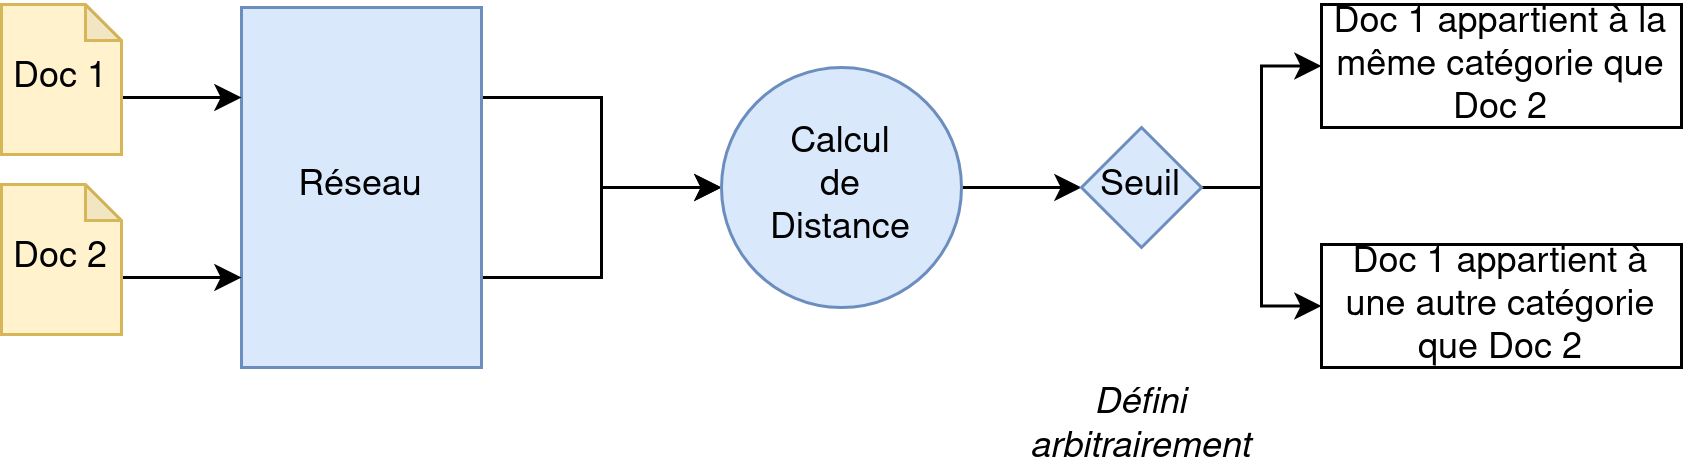
\includegraphics[width=\linewidth]{figures/chap4/Siamois.png}
    \caption{Architecture simplifiée d'un réseau siamois}
    \label{fig:chap4:structures:siamese-network}
\end{figure}

Malheureusement, les modèles de classification nécessitent en général un nombre conséquent de données d'entraînement pour être généralisables et donc dépasser le simple stade de preuve de concept. Si notre thématique est large et ses exemples répétés dans la littérature latine quelque soit la période, l'objectif n'est pas ici de ne proposer une solution qu'à la question sexuelle: d'autres thématiques pourraient intéresser d'autres chercheurs (par exemple, la paternité, les phénomènes météorologiques en mer, etc.) et une étude des limites quantitatives s'impose. On peut aussi s'intéresser à un découpage de notre isotopie en plusieurs sous-ensembles, soit du point de vue de la stylistique - usage métaphorique, explicite, comparatif, allusif -, des acteurs - femmes, hommes, enfants, esclaves, etc. - ou soit, encore, d'un point de vue moral - condamnation, neutre, positif. Qu'il s'agisse d'un autre thème ou d'une section du nôtre, l'usage du cycle apprentissage-prédiction-correction comme outil de constitution de corpus dès la dizaine, la centaine ou le millier d'exemples change le temps de travail nécessaire à cette compilation. Or, pour ce qui est des architectures neuronales, la classification par étiquette est connue pour ses limites sur de petits corpus\footnote{Bien qu'il s'agisse d'un corpus d'images, on peut trouver une étude relativement bien fournie sur une comparaison entre ces deux types d'outils: \cite{pasupa_comparison_2016}}. % Exemple ?

On s'intéresse alors à un autre mode de classification, celui par mesure de similarité et en particulier des modèles de réseaux siamois. Ces derniers incorporent la particularité de comparer au moins deux échantillons, dont l'un a une classe connue: après avoir produit une représentation numérique des échantillons, comme les modèles plus classiques, le réseau siamois est entraîné à réduire ou augmenter les distances entre ces échantillons afin de les catégoriser. À travers ces comparaisons, il va détecter plus rapidement les traits saillants des petites catégories. Cette architecture a le bénéfice d'être nettement plus efficace dans des situations dites de \textit{few-shot learning}, c'est-à-dire à faible set d'entraînement. 

Largement utilisé dans le domaine de la \textit{computer vision}, on en trouve un usage en histoire du livre à travers l'intéressant travail du projet Filigrane\footcite{shen_large-scale_2021} qui permet, dans des scores raisonnables, de classer facilement des filigranes papiers à partir de très peu d'exemples d'entraînement, mais y compris de potentiellement détecter des filigranes inconnus. Il est important de prendre en compte, lorsque l'on compare les scores des deux types d'architecture dans des publications différentes, la quantité des données d'entraînement: ces réseaux apprennent rapidement, pour des situations avec parfois de très nombreuses catégories. Dans un tel contexte, les modèles de classification ne proposent que rarement d'aussi bons résultats sans tomber dans le surapprentissage.

Avec un peu plus de deux mille exemples issus d'Adams, dans quel cas de figure se situe notre problème ? Si un tel set de données peut paraître important du point de vue d'un romaniste, il est en fait relativement bien faible comparé à des sets de données d'analyse de sentiment avec la pauvreté morphologique de l'anglais: assez petit, l'\textit{IMDB Movie Reviews Dataset}\footcite{maas-EtAl:2011:ACL-HLT2011}, un ensemble de critiques de films associées à des notes, ne compte \enquote{que} 50~000 exemples, à l'autre bout du spectre, l'\textit{Amazon Review Data}\footcite{ni_justifying_2019} en compte 233.1 millions. En regard de ces chiffres, notre modèle se limiterait-il à une recherche par similarité ? Rien n'est moins sûr, car, au contraire de l'exemple des filigranes, non seulement le nombre d'exemples pour une même catégorie est beaucoup plus élevé (les 2000 exemples relèvent de l'isotopie sexuelle), mais la variété à l'intérieur de ce set est beaucoup plus large: entre une métaphore militaire du courtisan d'Ithaque qui bande son arme et une claire mention d'\textit{irrumo}, la ressemblance est mince, tandis que deux prises de vue du même filigrane ont plus de points communs. C'est entre autres pourquoi nous nous appliquerons à évaluer la résistance des deux types d'architecture en fonction de plusieurs paramètres, y compris celui de la taille du set d'entraînement, dans l'optique de favoriser la construction \textit{ex nihilo} de futurs corpus sur d'autres thématiques.

% C'est une question importante, mais je me demande si ça arrive au bon endroit.

Question quelque peu laissée pour compte jusque-là, la question de l'unité syntaxique ou sémantique dans laquelle on souhaite identifier l'isotopie sexuelle reste assez centrale. On peut distinguer plusieurs niveaux allant de l'oeuvre à celui du mot. Le premier niveau, le niveau \textit{oeuvre}, pose un problème d'élasticité des tailles - entre un épigramme de deux vers de Martial et un livre de Tite-Live un monde existe - et d'utilité de l'outil: il n'est probablement pas intéressant de savoir si on parle de sexualité dans un livre d'historien romain, mais plutôt d'où se trouveraient de tels usages. Le deuxième niveau consisterait donc à détecter l'information au sein de petites séquences éditoriales comme des  \textit{paragraphes}, mais ils posent le problème de l'équivalence en poésie classique ou en théâtre: si un épigramme ou un court poème peut facilement être comparé à un paragraphe épistolaire de Cicéron en termes de taille, la question de leur équivalence en théâtre classique (une scène ? Une réplique ? Quid des répliques extrêmement courtes ?) ou en poésie épique semble difficile à résoudre. Ils restent alors séquences syntaxiques, représentées par des \textit{phrases} de l'éditeur, ou les unités qui les composent, les \textit{mots}, qui peuvent être intéressantes: la première forme une unité assez longue pour pouvoir développer des thématiques et la plus fine, dans un second temps, fournit une granularité à l'analyse. Cependant, cette unité syntaxique n'est pas sans inconvénient: comme le dit F. Rastier, le phénomène d'isotopie \enquote{est indépendant par principe des structures syntaxiques et de la prétendue limite de la phrase. Une isotopie peut s'étendre sur deux mots, sur un paragraphe, sur tout un texte.}\footcite[p. 34]{rastier_isotopie_1985}. Par exemple, si la mention claire de \textit{futuo} dans une phrase ne laisse pas de doute sur la thématique sexuelle, celle de l'allusion construite autour de la prise d'un chemin connu chez Ausone nécessite peut-être le texte en entier: d'ailleurs, ce morceau emprunté à Virgile (\textit{Aen.} 11.530) n'en avait pas le sens dans le contexte original; le jeune chef était Metebus, en exil avec sa fille. 

% Reprendre ici
\subsection{L'analyse de phrases en sciences humaines}

\subsubsection{La détection de métaphore: une tâche similaire ?}

Tâche formalisée plus clairement dans les années 2010, la détection automatique de métaphore partage avec notre tâche son échelle (l'information est recherchée au niveau phrase) et sa difficulté pour la machine (détecter les faisceaux de preuves qui indiquent un usage non littéral d'un certain nombre de mots). Il faut cependant prendre garder au sens qui est prêté à métaphore ici: dans leur ouvrage fondateur pour la partie traitement automatique du langage, \enquote{A Method for Linguistic Metaphor Identification}\footcite{steen_method_2010}, Steen et. al indiquent clairement s'insérer dans la tradition établie par Ortony, mais surtout Lakoff et Johnson\footcite{lakoff_metaphors_2003} dont les citations ponctuent le texte collectif. La définition anglo-saxonne utilisée relève ainsi plus de la détection d'usage figuratif du langage que d'un usage métaphorique au sens entendu en stylistique: "Sortir vainqueur d'un débat" serait ainsi une accumulation de métaphores, vainqueur empruntant au domaine du combat, et sortir du mouvement.

L'usage de cette définition de la métaphore conduit les auteurs à choisir le niveau du mot comme portant l'information quand ils établissent leur propre jeu de données, le \textit{VU Amsterdam Metaphor Corpus} (VUA\footcite{steen_method_2010}). Une compétition est ouverte pour la première fois en 2018 dans le cadre de la grande conférence NAACL sous le nom de \textit{Shared Task on Metaphor Detection}\footcite{leong_report_2018}. Ce système de compétition est assez commun dans le monde du TAL et de l'intelligence artificielle en général: il s'agit, quelques mois avant une conférence (ici cinq), de fournir un set de données d'entraînement, de demander aux équipes de fournir soit un script permettant d'annoter des données tests, soit d'annoter, sans connaître la vérité de terrain, ces données puis d'obtenir le classement au moment de la conférence. Cette compétition utilise alors le set de données cité précédemment, et retient le \textit{F1-Score} comme méthode de mesure: la présence d'un set particulièrement déséquilibré - il y a plus de mots sans usage figuratif - favorise l'usage d'un outil laissant plus de place aux erreurs dans le décompte final. Durant cette compétition, le seul outil n'utilisant pas de réseau neuronal profond (DNN) est classé dernier sur toutes les tâches. En tête de l'ensemble des tableaux, deux des trois outils utilisent en plus d'informations sémantiques portées par des \textit{embeddings} des informations morphosyntaxiques, l'annotation POS des mots. Le papier \textit{bot.zen}\footcite{stemle_using_2018} utilise par ailleurs plusieurs \textit{embeddings} différents, certains entraînés sur des corpus de personnes en cours d'apprentissage de la langue anglaise\footnote{Les auteurs s'appuient sur l'hypothèse d'une surreprésentation d'un langage figuratif chez les personnes apprenant une nouvelle langue, \textit{cf.} \cite{klebanov_argumentation-relevant_2013}}. 

Une seconde compétition a eu lieu en 2020\footcite{leong_report_2020} dans le cadre de la conférence ACL. Cette compétition voit logiquement l'arrivée massive des \textit{transformers} (RoBERTa, Bert, Albert, etc.) dans le domaine, et ces architectures prennent constamment au moins les 5 premières places sur les 12 participants retenus. Le meilleur des modèles, \textit{DeepMet}, propose encore une architecture utilisant des embeddings, cette fois issue de transformers, et des informations morphosyntaxiques (deux formes de POS). Le F1-Score reste l'élément principal pour évaluer les contributions et les meilleurs scores atteignent 76.9\% toutes catégories morphosyntaxiques confondues sur le dataset VUA. Pour aller plus loin dans la compréhension de ce que peuvent apprendre ces algorithmes, ces deux compétitions se sont intéressées au taux de succès en fonction des genres (Académique, Fiction, Presse, Conversations) et à l'écart de performance en fonction de ceux-ci. % Et ? Ajouter quelque chose ?

La relation entre cette tâche et les études littéraires ou la stylistique est cependant bien ténue: le seul lien que l'on puisse faire est celui de la présence d'une personne identifiée comme faisant partie du domaine des humanités numériques, J. B. Herrmann, parmi les auteurs du corpus VUA et de l'ouvrage collectif fondateur\footcite{steen_method_2010}. Peu de publications réutilisent la notion du côté SHS, J. B. Hermann ne proposant elle-même qu'une publication autour de ce thème, une analyse quantitative des métaphores dans le registre universitaire\footcite{herrmann_high_2015}. Et des outils issus de cette compétition, il ne semble qu'aucun n'aie vu un usage en SHS. Comme beaucoup de recherches en TAL, l'usage de ces modèles développés dans le cadre de ces \textit{workshops} est mince dans des recherches littéraires. Ainsi, si les auteurs de \textit{Metaphor Detection in a Poetry Corpus}\footcite{kesarwani_metaphor_2017} s'intéressent aux capacités de transfert d'apprentissage entre un corpus poétique et non poétique, il ne s'intéresse pas à la réutilisation de cette méthode pour classer les auteurs en fonction de leur usage figuré du langage. Cette absence d'intérêt pour des analyses littéraires quantitatives montre bien cette forme d'isolement qui peut se produire autour du TAL, focalisé sur la linguistique et l'obtention du meilleur score. Il est pourtant facile d'imaginer une application de ces modèles, dans le milieu francophone: nous pourrions, pour des auteurs du 20e siècle, étudier si un usage figuratif du langage sépare les auteurs s'opposant au surréalisme, comme l'annonce distinctement Jules Supervielles dans son \textit{En songeant à un art poétique}, à ces surréalistes; ou encore, nous pourrions tout autant analyser si le langage figuratif est un critère de style pour les auteurs ayant baigné dans plusieurs genres, comme Jean-Paul Sarte ou Albert Camus.

\subsubsection{L'attribution d'auteur}

Loin des questions métaphoriques, celle de l'attribution d'auteur est un domaine particulièrement présent en philologie classique: à travers la transmission des textes, l'autorité a parfois été perdue (textes anonymes), modifiée (textes remaniés), créée (faux de l'antiquité tardive et du haut moyen-âge) et enfin noyée (textes composites). De la question homérique à l'identité des auteurs préfixés habilement par \texttt{Pseudo} en passant par les dizaines de sermons douteusement attribués à Augustin et Chrysostome, la recherche d'autorité est une tradition qui s'est longtemps basée sur une connaissance d'experts et une analyse fine de quelques passages, notamment en cherchant des informations permettant de postdater un texte à la mort de son auteur par exemple. 

Cette question de l'attribution d'auteur a par ailleurs la particularité d'avoir un vrai retentissement médiatique: si la question homérique ne passionne plus les médias de masse - l'a-t-elle jamais fait ? -, celle de l'autorité shakespearienne ou moliérienne passionne encore aujourd'hui\footnote{En 2019, via une publication de J.B. Camps et F. Cafiero sur le sujet, la débat a été clôt - ou relancé, au choix - et a atteint les rédactions de grands journaux français (le Figaro, le Point), les radios (France Culture) et jusqu'au plateau de télévision (BFM-TV}. L'anonymat d'un auteur - comme celui de J. K. Rowling\footcite{juola_how_2013} - ou l'hypothétique subterfuge de l'auteur connu qui aurait utilisé des plumes anonymes passionnent: l'enquête policière rentre ainsi dans le débat littéraire. Et c'est bien l'incursion de la statistique, et en particulier celle via ordinateur, qui a complètement changé la donne. 

De premières publications dans les années 50 et 60, la stylométrie, c'est-à-dire la quantification du style, a connu dans le monde des humanités numériques un véritable pic aux à partir de 2015 (jusqu'à 10\% des conférences en humanités numériques, \textit{cf.} Figure \ref{fig:chap4:attribution-auteurs}). Mais si toute attribution d'auteur n'est pas stylométrie et inversement, il convient de séparer aussi la première des catégories en deux sous-catégories: la découverte d'auteur (\textit{authorship verification}), une méthode en général non supervisée , qui cherche à faire des regroupements d'autorité sans présumer des individus impliqués (par exemple, chercher à identifier les différents auteurs dans l'Anthologie Latine), et l'attribution d'auteur (\textit{authorship attribution}) à proprement parler, méthode supervisée avec l'intention d'entraîner la machine à reconnaître des auteurs en particulier.

Dans le domaine classique, quatre articles retiennent notre attention par la diversité de leurs approches. L'article de Kestemont et al.\footcite{kestemont_authenticating_2016} sur le corpus césarien approche la problématique comme une question ouverte, et conclue à l'existence possible de 5 auteurs: la méthode se base sur les propriétés textuelles classiques de la stylométrie, sélectionnant ainsi les unigrammes de mots et n-grams de caractères les plus fréquents du corpus, en normalisant leur présence et en projetant l'ensemble dans un espace contraint. Il s'inscrit dans un renouveau du domaine stylométrique après 2015 et intègre un plus gros réseau de publications et d'interventions où les principaux acteurs, Kestemont, Eder et Rybicki, sont aussi les auteurs de l'outil popularisant la méthode, stylo\footcite{stylo_r}. %

L'article de R. Gorman\footcite{gorman_author_2020} s'intéresse quant à lui à l'utilité de la syntaxe avançant l'hypothèse que, contrairement à l'information lexicale, cette information est susceptible de mieux résister aux différences génériques et thématiques. Il approche la question sous l'angle de la vérification: une fois les propriétés sélectionnées parmi les informations morphologiques et de dépendance, la représentation vectorielle de chaque texte est transmise à un réseau décisionnel (SVM ou régression linéaire) avec des résultats allant de 85\% à 100\% de réussite.

L'article de B. Nagy\footcite{nagy_metre_2021} s'intéresse de la même manière à des propriétés non lexicales, mais ne s'intéresse pas à l'information syntaxique pour autant: ici, c'est la construction des hexamètres, à travers les césures, les accents, les combinaisons de dactyles et de spondées, qui informe la décision finale, faite par quatre algorithmes différents, mais dont les deux plus performants sont SVM et une régression linéaire. Les scores sont particulièrement élevés, mais l'auteur lui-même émet des réserves: le mètre n'est qu'une facette du style, et il n'est pas improbable qu'une situation de surapprentissage ait lieu. Par ailleurs, sa méthode n'est pas robuste à un changement de style volontaire et stylistiquement plausible. Enfin se pose la question de l'impact des choix d'éditeurs qui - parfois - choisissent aussi la forme qui leur semble la plus cohérente stylistiquement et métriquement parlant, et qui favoriserait d'une certaine manière le choix d'auteur. 

Enfin, le dernier article de Vanni et al.\footcite{vanni_textual_2018} ne s'intéresse pas directement ni à une question de style, ni à une question philologique, mais plutôt à la possibilité de proposer un meilleur réseau d'encodage pour la vérification d'auteur. Comme les deux précédents, il s'inscrit dans la logique de vérification d'auteurs, mais est le seul à introduire une approche par réseau neuronal via projection, encodage et couche décisionnelle. C'est aussi le seul article qui ne filtre pas l'information initiale par des seuils de présence: dans le cadre de la vérification d'auteur, une telle absence de seuil peut introduire des variations thématiques comme outils de séparation. Ces variations thématiques fonctionnent bien sur un corpus fermé (César peut parler de Cicéron, mais pas de Domitien, Domitien sera donc une propriété négative pour la reconnaissance de César), mais sur un corpus plus rapproché dans le temps et uni du point de vue générique et thématique, le fonctionnement du modèle laisse peu de doute sur sa propension à se focaliser sur ces traits saillants du lexique et à ignorer ainsi les traits de style.

Bien que la vérification d'auteur soit une tâche de classification de texte, il est intéressant de voir qu'elle a la particularité de reposer souvent le masquage de l'information lexicale générique et thématique pour faire ressortir le stylome: cette suppression d'information est à l'opposé de la tâche qui nous intéresse. Cependant, l'intérêt des informations syntaxiques relevé par les deux articles de Gorman et Nagy doit être évidemment pris en compte, d'autant plus qu'il répète des besoins relevés par la recherche en détection de métaphores où la POS améliorait les scores.

\subsubsection{L'intertextualité: un domaine central de philologie computationnelle}

% Reprendre ici, premiers paragraphes gérés mais y a une duplication de vetus latina

L'intertextualité, ou l'étude des \enquote{transferts de matériaux textuels à l'intérieur de l'ensemble des discours\footcite{aron_intertextualite_2010}}, a trouvé dans les études quantitatives et numériques en général un nouveau souffle. Domaine formalisé dans les années 1960, il n'en est pas moins une tâche pluriséculaire de recherche de connexions entre plusieurs textes: on peut ainsi trouver dans le travail des scoliastes médiévaux et des éditeurs de la patrologie de Migne des chercheurs d'intertextualités lorsque, face à un texte de père de l'Église, ils s'efforcent de retrouver pour chaque passage, chaque allusion ou citation, la source biblique utilisée. Tant est que c'est à travers ce travail d'annotation que l'on finit par produire une - puis des - \textit{vetus latina}, bibles composites reprenant les citations de versions de la Bible supplantées par la \textit{Vulgate}. Bien que \enquote{l'intertextualité ne se [limite] pas à une série de citations ou d'allusions repérables}\footcite{aron_intertextualite_2010}, c'est plutôt cette branche qui intéresse dans un premier temps la recherche quantitative sur corpus - et pour cause, la détection de \enquote{clichés et de stéréotypes} est aussi plus difficile pour le lecteur humain. Les manifestations d'intertextualité relevant de la citation ou de l'allusion sont très clairement impossibles à ignorer dans la tradition du commentaire, religieux ou non, présent dans la littérature latine à travers les premiers ouvrages chrétiens, mais aussi les grammairiens ou commentateurs tels que Donat ou Porphyrion: pour Donat, le texte dans les éditions transmises est clairement cité, pour les pères de l'Église, les citations ou allusions sont le coeur des ouvrages. 

Par ailleurs, ce travail de citation entre auteurs est lui-même un angle d'étude pour la littérature latine et grecque\footcite{darbo-peschanski_citation_2004}: on peut penser, à trois siècles d'écart, à la citation directe de Martial par Ausone (\enquote{\textit{Lasciva est nobis pagina, vita proba}}\footnote{\enquote{Notre page est lascive, notre vie probe.}}) dans ses propres épigrammes qui peut lui permettre d'introduire un avertissement au lecteur. Cette pratique gréco-latine de la citation est telle qu'elle permet d'ailleurs de reconstituer, même à l'état de fragment, les oeuvres perdues, de la \textit{Vetus Latina} aux oeuvres d'Accius citées par Priscien, Festus, Macrobe, etc. La période antique relève donc de la véritable mine d'or pour le développement de modèles automatiques de reconnaissance de citation, car elle propose des corpus qui ont déjà été de maintes fois étudiées, tant est que de "petits" projets comme le \textit{Digital Fragmenta Historium Graecorum} atteignent 7256 fragments tandis que le plus gros d'entre eux, \textit{Biblindex}, représente 370.000 références vérifiées et inscrites. Historiquement, il est intéressant de remarquer que le même lieu qui accueillait le colloque de C.  Darbo-Peschanski en 2004 est celui qui réunit pour la première fois - à notre connaissance - ce domaine computationnel et celui des belles lettres à travers la journée d'étude \textit{International Workshop on Computer Aided Processing of Intertextuality in Ancient Languages} qui a eu lieu du 2 au 4 juin 2014 à Lyon, ville qui héberge aussi le projet \textit{Biblindex}.

L'\textit{intertextualité quantitative}, dont C. W. Forstall et W. J. Scheirer figent le nom en 2019\footcite{forstall_quantitative_2019}, ne prend cependant pas toutes ses sources dans l'étude de l'antiquité. Au contraire, un autre phénomène intéresse ce domaine: la question de la détection du plagiat. Bien sûr, et ils le citent, le centon est probablement l'une des premières oeuvres plagiaires, mais la notion de \enquote{d'invention n'est pas le critère discriminant de la valeur littéraire avant le XVIIIe siècle}\footcite{aron_plagiat_2010}: si le mot \textit{plagiarus} existe, il ne concerne pas à la réutilisation de morceaux de texte mais le vol d'autorité (Martial, I.53). Mais l'histoire du plagiat, de la circulation des textes et de leur remaniement ne s'arrête pas au 4e siècle de notre ère: au contraire, cette question peut se relever particulièrement intéressante lorsqu'elle commence à toucher les médias de masse telle que la presse. À travers le projet de D. Smith par exemple\footcite{smith_computational_2015, smith_infectious_2013}, dès 2013, on retrace la propagation aux États-Unis de textes - tels que des recettes de cuisine, des dépêches, des petites histoires - dans la presse. Cependant, sans en dénier la difficulté, surtout au début des années 2000, un monde existe entre la détection de textes entiers légèrement remaniés dans la presse américaine et la détection même discutable d'intertextualité telle que l'allusion virgilienne par Ovide que mentionnent Forstall et Scheirer en introduction (\textit{Arma gravi numero violentaque bella parabam Edere}, Ov. \textit{Am}. 1.1). 

% Dois-je définir allusion, citation. réécriture ? Pas envie...

Mais quel niveau de difficulté présente ce domaine ? D'un point de vue humain, la détection d'allusion reste toujours sujette à débat, et si les mentions virgiliennes par Ovide ou martialienne par Ausone sont sans équivoque, restent de nombreux passages où la mention fait question, et où certains verront dans la simple présence d'un mot solitaire une intertextualité marquée avec un autre auteur. Mais du point de vue humain comme du point de vue de la machine, le problème réside aussi dans les dimensions du problème: de la recette de cuisine remaniée transmise de journal à journal à l'incipit des \textit{Amours} ovidiennes, le problème de l'intertextualité réside dans le fait que tout peut être source d'intertextualité, et que tout peut faire mention. Pour tout ensemble de mots, du simple mot au texte entier pour la presse du XIXe siècle américain, il existe potentiellement une unité\enquote{source} dans l'ensemble de la production littéraire de même langue - voire de langue étrangère - qui la précède. Même pour le corpus latin transmis du 2e siècle, cela représente plusieurs millions de mots et autant de séquences à la taille indéfinie. Cette tâche de minage de corpus s'apparente alors à la recherche d'information (\textit{information retrieval}) plus qu'à la simple classification.

Du point de vue technique donc, il ne s'agit pas des mêmes méthodes que la détection de métaphore vue précédemment. L'intertextualité quantitative est passée respectivement du \textit{fuzzy matching} - une recherche de correspondance partielle de chaînes de caractères - à la mesure de similarité via des réseaux neuronaux. Pour l'étude des textes anciens en latin, le projet \textit{Tesserae}\footcite{coffee_tesserae_2013} s'intéresse principalement à la présence dans un passage d'une taille définie (d'un à plusieurs vers) des mêmes lemmes, quelques soit les différences de flexion, soit par l'usage de lemmatisation, soit par l'usage de stemmes, résultat de la découpe du lemme à la racine. Cette approche se limite donc à l'intertextualité \enquote{lexicale} telle que définie par C. W. Forstall\footcite{forstall_quantitative_2019} mais produit non seulement de nouvelles données (seule la moitié des intertextualités reconnues par Tesserae chez Lucain sont connues des commentateurs modernes), mais aussi de nouvelles pistes de réflexion sur l'objet étudié: on sort de l'exploit technique et on réintroduit des intérêts littéraires dans l'analyse quantitative. 

Pour passer de la détection d'intertextualité lexicale, qui partage des lemmes, à l'intertextualité sémantique, qui partage des sèmes, le passage à d'autres techniques de calcul est nécessaire. Dans leur manuel, Forstall et Schreier utilisent simplement la \textit{Latent Dirichlet Allocation} (LDA) - une technique liée au \textit{topic modeling} et des calculs de similarité à base de distance cosinus pour relier les passages entre eux. D'un point de vue technologique, c'est d'ailleurs étonnant que, malgré une publication en 2019, ces derniers parlent des projections Word2Vec ou GloVe comme de futures applications: les techniques d'embeddings citées datent du tout début des années 2010, 2019 voyant l'apparition des technologies de \textit{transformers}. 

Il semble en effet que la prochaine étape pour l'intertextualité quantitative soit de briser la barrière de l'allusion fine, où le partage sémantique est faible entre le passage cité et le citant. Dans leur article \textit{On the Feasibility of Automated Detection of Allusion\footcite{manjavacas_feasibility_2019}}, les auteurs s'intéressent à la situation propre de cette catégorie, et montre une forte différence de difficulté avec la détection de citation complète ou d'intertextualité lexicale en général: dans le set de données utilisé, des sermons annotés de Clairvaux, pour les allusions, seuls 6\% des formes et 12\% de lemmes sont partagés avec le texte référence, soit respectivement 4 et 3 fois moins que les autres catégories d'intertextualité que catégorise L. Mellerin à Biblindex. Architecturalement, le modèle final le plus performant est un modèle hybride, mêlant informations lexicales et sémantiques, utilisant la projection de mot \textit{FastText} sur un texte lemmatisé. Cet usage de \textit{FastText}, et sa primeur face à \textit{Word2Vec}, sont intéressants, car \textit{FastText} est connu pour capturer moins bien la proximité sémantique que d'autres formes d'\textit{embeddings} tout en capturant mieux les groupes de mots (par exemple \textsc{lascivus} et \textsc{lascivo}) et les relations syntaxiques\footcite{hartmann_portuguese_nodate}. Mais les résultats sont loin d'être satisfaisants, les auteurs admettant eux-mêmes que la marche reste longue: au mieux, pour moins de la moitié des exemples, la bonne réponse se trouvait dans le top 20 des résultats de la recherche. 


\subsection{Des tâches sans rapports ? De la classification d'article sur eBay à la détection de harcèlement dans le monde du jeu vidéo}

% Reprendre ici

Si certaines applications de la recherche en traitement automatique des langues croisent régulièrement les intérêts des sciences humaines, d'autres peuvent sembler bien étrangers. Et pourtant, qu'il s'agisse de moyen (classification), de difficulté (information implicite ou explicite) ou de thème (sexuel), on peut trouver dans les recherches actuelles quelques problématiques qui peuvent aiguiller notre propre recherche du point de vue architecture comme de celui de la mesure des résultats. 

Sur les réseaux sociaux comme dans le monde du jeu vidéo, la question de la modération quasi instantanée des contenus, en particulier ceux impliquant une forme de harcèlement ou des contenus sexuellement explicites, est devenue un véritable enjeu. Pour les deux types d'espaces d'échanges, et en particulier pour ceux des jeux massivement multijoueurs, la gestion de la toxicité des plates-formes et sa réduction sont des conditions \textit{sinequanone} d'un maintien d'une communauté d'utilisateurs actifs. Si chaque partie d'un jeu était un torrent d'insultes, la base de joueurs réguliers tendrait logiquement à se réduire, de même que les bénéfices de l'éditeur du dit jeu, particulièrement pour les jeux gratuits à l'installation qui tirent leurs bénéfices d'achats de bonus (éléments esthétiques, fonctionnalités supplémentaires, etc.) sur une longue durée. 

Ces problématiques se lient rapidement à la question de l'apprentissage machine pour deux raisons: d'une part, il permet une gestion en flux des \enquote{délits} de contenus; d'autre part, il réduit les coûts humains de la modération\footnote{À laquelle ils sont tenus légalement dans de nombreux pays.} manuelle des contenus, potentiellement extrêmement importants pour des plates-formes aussi grosses que Twitter par exemple. Pour \textit{League of Legends}, un jeu paru fin des années 2000, des chercheurs établissent en 2014\footcite{blackburn_stfu_2014} une méthode de capture de mots à partir d'un dictionnaire de valeurs, l'\textit{Affective Norms for English Words}\footcite{bradley_affective_1999}, et d'informations liées à la partie indiquée comme problématique. Parmi les informations utilisées par l'algorithme, un simple \textit{Random Tree Forest}, celles des messages et de la polarité (\textit{valence} en anglais) des termes employés, représentent trois des cinq informations contribuant le plus à la décision finale de punir ou d'innocenter une personne indiquée comme toxique par ses partenaires temporaires de jeu. Cependant, les dictionnaires de polarité posent le problème du contexte: "Toi au moins, tu n'es pas [TermeInsultant]" ne serait pas un abus de langue, tandis que "Toi au moins, tu n'es pas [TermeInsultant] contrairement à [NomDePersonne]". Sept ans plus tard, la recherche a intégré d'autres modèles d'information tentant de réduire cette limite: dans leur article \textit{Automatically Detecting Cyberbullying Comments on Online Game Forum}\footcite{vo_automatically_2021}, les auteurs comparent les performances de modèles à propriétés (\textit{features} soumises à SVM et aux régressions linéaires), à encodage après projection (projections via [Glove, fastText] puis encodage avec [CNN,GRU]) et à projection par \textit{transformer} (Toxic-BERT). Les résultats sont mesurés par F-Score à cause du déséquilibre des sets de données (beaucoup moins de données positives que négatives) et donnent lieu à de véritables bonds entre les différentes technologies: de 50\% de F-Score pour les premiers modèles, les seconds atteignent 75 à 80,7\% tandis que le modèle à base de \textit{transformer} atteint 82,7\%. On note un très faible écart entre les modèles Text-CNN+Glove et le modèle à base de Toxic-Bert, tout juste 2\% sur les données issues du jeu League of Legends, tandis que seul 0,76\% les séparent sur celles du jeu World of Warcraft.

Dans la catégorie de classification de textes, la question de la détection de l'isotopie sexuelle peut se manifester sous d'autres traits. De la détection automatique de prédateurs sexuels à la classification de chansons pour leur commercialisation, le contenu explicitement ou implicitement sexuel pose plusieurs problèmes en fonction du contexte de recherche. Pour la prédation sexuelle, la problématique glisse vers l'implicite et la détection de progression discursive. Dans ce contexte, il semble que la compétition du PAN\footnote{\textit{Plagiarism Analysis, Authorship Identification, and Near-Duplicate Detection} - http://pan.webis.de/} de 2012 \textit{Sexual Predator Identification}\footcite{inches_overview_2012} constitue encore le plus gros dataset existant. Comme pour notre dataset, les données sont - heureusement - déséquilibrées en faveur de contenus non problématiques, avec seulement 4\% de conversations marquées comme contenant une prédation. On distingue pour ce domaine les mêmes évolutions que pour celui de la toxicité, à savoir un passage d'un modèle \textit{Bag-Of-Words} avec des dictionnaires de valeurs vers des modèles d'apprentissage profond, avec une évaluation via le F1-Score. Parmi les modèles les plus récents, celui de Muñoz et al.\footcite{munoz_smartsec4cop_2020} utilise une projection via \textit{Word2Vec} puis un encodage via des réseaux convolutionnels de filtres de taille 2 à 5, mais ses résultats en F1 sont particulièrement bas (environ 40\%). Au contraire, Vogt et al.\footcite{vogt_early_2021} atteint entre 89 et 80\% en utilisant une projection via Bert et en prenant optionnellement en compte la dimension temporelle d'une discussion, et donc, sa progression discursive. 

Dans une dimension plus légère, la classification des contenus explicites des paroles de chanson pose un problème pour leur commercialisation et leur mise en écoute libre sur des plates-formes comme Amazon, Youtube ou Spotify chez les mineurs, particulièrement aux États-Unis avec la mise en place du \textit{Parental Advisory Label} qui requiert l'annotation de ces messages. Les membres du projet WASABI proposent un récapitulatif des méthodes, mises au banc d'essais sur un dataset fraichement formalisé, via les mêmes techniques que les applications précédentes, à savoir une attaque par dictionnaire, une attaque par \textit{Bag-Of-Word}, un réseau utilisant des CNN et une projection via des \textit{embeddings}, un modèle inédit pour la littérature étudiée ici à savoir un réseau récurrent avec attention (HAN) et enfin un modèle BERT. De cet article, plusieurs conclusions des auteurs sont intéressantes:
\begin{itemize}
    \item Le modèle convolutionnel brille face à l'ensemble des autres modèles pour la catégorie explicite avec un score de 63\%.
    \item Le modèle Bert surpasse les autres sur la catégorie non explicite, majoritaire dans le corpus (90\% des exemples).
    \item Les différences de score restent particulièrement minimes (quelques points d'écart) suivant les catégories, quelleque soit l'architecture.
    \item Plus important encore, le modèle semble se spécialiser dans la détection du contenu explicite en Hip-Hop, et les auteurs posent justement la question du biais du set de données ou de la possibilité de surapprentissage du modèle sur ces traits facilement reconnaissables.
\end{itemize}
De manière assez intéressante, contrairement aux travaux en détection de métaphore, aucune information grammaticale ne semble avoir été intégrée au réseau, alors même que les auteurs indiquent le problème de la bivalence grammaticale verbe/nom du mot \textit{bitch} (fr. salope) qui peut comprendre aussi le simple sens \enquote{se plaindre} de manière vulgaire. Par ailleurs, ils notent aussi que le simple usage d'une vulgarité explicite comme \textit{bitch} dans une chanson telle que celle de Meredith Brook est alors prise à contre-courant, pour se réapproprier le sens et le questionner: il devient alors un sujet de la chanson et se défait en partie de sa connotation vulgaire.

Pour finir, la classification de texte peut devenir un problème particulièrement complexe lorsque le nombre d'exemples est particulièrement bas, moins d'une dizaine par exemple, et le nombre de catégories élevé. Cette problématique se retrouve particulièrement dans le domaine du marketing web où les catalogues sont crowdsourcés, tel eBay, ou pour les agrégateurs de contenu, tels Google News. Historiquement, en 2007, la génération de ces rapprochements pour les flux tels que Google News a principalement été opérée dans un contexte de classification non supervisé, via des méthodes de clustering ou d'indexation latente\footcite{das_google_2007}: il s'agit alors à la fois de regrouper des événements, mais aussi d'intégrer à cette classification une forme de personnalisation des résultats. Il existe bien sûr des outils internes, tels que ceux développés par Reuters\footcite{nugent_comparison_2017}, pour détecter des catégories précises, mais la classification instantanée d'informations nouvelles reste majoritairement une question de mesure de proximité entre des projections de document. 

Parallèlement, on retrouve ces problématiques dans le catalogage de masse de boutiques crowdsourcées telles qu'eBay. Dans ce cadre, la classification par réseau siamois semble apporter un avantage considérable\footcite{shah_neural_2018}. En effet, non seulement le nombre d'exemples est extrêmement faible  - parfois, un nouveau produit émerge, donnant ainsi lieu à une classification à 0 exemple - mais le nombre de classes extrêmement élevé (de l'ordre du million). Les modèles proposés utilisent alors une projection via FastText\footcite{fasttext}, un encodage via un LSTM bidirectionnel de 3 couches et les décisions prises sur la base d'une mesure de distance euclidienne. Les résultats varient alors de 82 à 97\% d'\textit{accuracy} en fonction des catégories, la catégorie "Vêtements, chaussures et accessoires", probablement la plus variée, obtenant le score le plus bas.

\subsection{Résumé des architectures rencontrées}

Après cette revue des différentes tâches qui s'apparentent à la classification de texte, il est intéressant de remarquer une véritable constante: presque tous les modèles reposent sur une structure Projection-Encodage-Décision où la couche de décision peut-être au choix une régression linéaire ou bien une mesure de similarité. Évidemment, chaque tâche intègre ça et là des variations, par exemple la prise en compte de la progression de discussion, mais la structure générale des éléments d'encodage reste la même. Il est par ailleurs intéressant de voir largement utilisée la mesure du F1-Score pour l'ensemble des tâches à labels déséquilibrés. On remarque aussi un véritable changement du domaine sur la décennie 2010-2020, avec  d'abord l'avènement des projections de mots aux alentours de 2013 grâce à \textit{Word2Vec} et \textit{GloVe}, à l'apparition de nouveaux systèmes de classification dans le domaine du traitement textuel (réseaux siamois) vers 2017/2018, la diversification des couches d'encodage, du LSTM au CNN, y compris modifiés, et enfin à la fin de la décennie, le changement profond qu'apporte Bert et les transformers pour les langues modernes. Cependant, il reste intéressant de voir la résistance de certains modèles dans quelques cas de figure (stylométrie par exemple ou classification de chanson) qui résistent plus que correctement aux changements technologiques et aux différences de coût qu'ils impliquent.

% Rajouter un cas d'étude ici en Siamese ?


\section{Développement des architectures et mise en place des modèles}

\subsection{Du corpus aux données d'entraînement et d'évaluation}

Avant de pouvoir produire des modèles, la transformation du corpus de recherche en jeu de données d'entraînement est nécessaire. Celle-ci passe par plusieurs étapes: il faut passer d'un format de conservation à un format d'exploitation, il faut contrebalancer les données \enquote{unicatégorielles} (classe \texttt{isotopie-sexuelle}) par des données ne présentant pas cette isotopie.


\subsubsection{Formats des fichiers, simplification des données}

\begin{figure}
    \centering
    \begin{adjustbox}{width=0.9\textwidth,keepaspectratio}
    \lstset{language=XML}
    \begin{lstlisting}[language=XML]
<div type="fragment" ana="#acte #fututio">
  <bibl ref="#adams">
      <author>J. N. Adams</author>,
      <title xml:lang="lat">The Latin Sexual Vocabulary</title>,
      <biblScope unit="page">119</biblScope>
    </bibl>
    <bibl type="source">
        <author>
            <persName xml:lang="fr">Catulle</persName> [<persName xml:lang="eng">Catullus, Gaius Valerius</persName>]
            <idno type="VIAF">https://viaf.org/viaf/100218993/</idno><idno type="LC">n79-6943</idno>
        </author>,
        <title xml:lang="lat">Carmina</title>,
        <biblScope unit="ref">6.13-6.14</biblScope>
        <idno type="CTS_URN">urn:cts:latinLit:phi0472.phi001.perseus-lat2</idno>
    </bibl>
    <quote xml:lang="lat" source="urn:cts:latinLit:phi0472.phi001.perseus-lat2:6.13-6.14" type="line">
    <w ref="6.13" lemma="non" pos="ADVneg" 
      msd="MORPH=empty">non</w>
    <w ref="6.13" lemma="tam" pos="ADV" 
      msd="Deg=Pos">tam</w>
    <w ref="6.13" lemma="latus1" pos="NOMcom" 
      msd="Case=Acc|Numb=Plur">latera</w>
    <w ana="#acte #fututio" ref="6.13" lemma="effutuo" pos="VER" 
      msd="Case=Acc|Numb=Plur|Gend=Neut|Mood=Par|Tense=Perf|Voice=Pass">ecfututa</w>
    <w ref="6.13" lemma="pando2" pos="VER" 
      msd="Numb=Sing|Mood=Sub|Tense=Pres|Voice=Act|Person=2">pandas</w>
    <w ref="6.13" lemma="," pos="PUNC" 
      msd="MORPH=empty">,</w>
    <w ref="6.14" lemma="ni2" pos="CONsub" 
      msd="MORPH=empty">ni</w>
    <w ref="6.14" lemma="tu" pos="PROper" 
      msd="Case=Nom|Numb=Sing">tu</w>
    <w ref="6.14" lemma="quis1" pos="PROint" 
      msd="Case=Acc|Numb=Sing|Gend=Neut">quid</w>
    <w ref="6.14" lemma="facio" pos="VER" 
      msd="Numb=Sing|Mood=Sub|Tense=Pres|Voice=Act|Person=2">facias</w>
    <w ref="6.14" lemma="ineptiae" pos="NOMcom" 
      msd="Case=Gen|Numb=Plur">ineptiarum</w>
    <w ref="6.14" lemma="." pos="PUNC" 
      msd="MORPH=empty">.</w>
  </quote>
</div>
    \end{lstlisting}
    \end{adjustbox}
    \caption{Exemple de ressource en XML pour l'entraînement}
    \label{fig:xml-model-example}
\end{figure}

En premier lieu, afin d'assurer la réutilisabilité des données, il est nécessaire d'expliquer les diverses transformations qu'elles ont subies pour devenir jeu de données pour l'entraînement de modèles. Le format du corpus pour leur conservation et exploitation \enquote{manuelle} consiste en un ensemble de fichiers XML (\textit{cf.} Figure \ref{fig:xml-model-example}) contenant à la fois les informations grammaticales sur chaque mot (lemme, POS, annotations morphosyntaxiques), l'analyse des termes centraux portant les sèmes actualisés de l'isotopie, les métadonnées sur l'extrait (auteur, oeuvre, identifiant de passage) et les diverses annotations issues de la lecture d'Adams (champs lexicaux, figure de style employée, etc.). Si les données XML sont particulièrement adaptées à la réexploitation de corpus, nous faisons le choix de convertir ce corpus vers un nouveau format permettant une lecture plus rapide des données. Le format de sortie, dont un extrait est présenté en figure \ref{code:chap4:training-data-format}, est une forme de TSV personnalisé et propose quatre types de lignes:
\begin{itemize}
    \item Le premier type commence par \texttt{[header]} est tout simplement la ligne d'en-tête, où chaque colonne qui suivra dans le TSV est nommée. Elle inclut ainsi les noms des colonnes \textit{token}, \textit{lemma}, etc. Pour une exploitation plus fine de la morphologie (genre, nombre, cas, mode, temps…), l'information rassemblée dans un seul élément\texttt{@msd} du fichier XML est désormais réorganisée dans le tsv avec une colonne pour chaque trait grammatical.
    \item Le second type de ligne est celui de division des échantillons: chaque phrase échantillon est séparé par une à plusieurs lignes vides.
    \item Le troisième type de ligne concerne le contenu des échantillons: chacun de leurs \textit{tokens} est représenté par une ligne en suivant le format et l'ordre de l'en-tête. Les enclitiques et les phénomènes d'élision du type \textit{est → -st} sont alors représentés par une duplication de la forme entourée des caractères \texttt{\{\}} ou bien une forme indépendante (pour \texttt{-ne, -que, -cum et -ve}) avec son analyse grammaticale propre. Les formes les plus communes ont pu être capturées de cette manière, les autres sont donc dédoublées.
    \item Le quatrième type concerne les métadonnées: qu'elles soient activables (intéressante pour la classification) ou descriptives (afin de pouvoir mieux analyser les résultats), ces lignes de métadonnées commencent nécessairement par un \texttt{\#} ou par un \texttt{[}. Un échantillon commence nécessairement par une ligne indiquant sa catégorie (\texttt{\#[TAG]positive} ou \texttt{negative}). 
\end{itemize}

\begin{figure}
\centering
\begin{adjustbox}{width=0.9\textwidth,keepaspectratio}
\begin{lstlisting}

[header]	token	lemma	pos	Case	Numb	Gend	Mood	Tense	Voice	Person	Deg
#[TAG]negative
[GENERIC-METADATA]urn=urn:cts:latinLit:phi1318.phi001.perseus-lat1
[GENERIC-METADATA]fp=./dataset/negative-examples/latinLit_phi1318.phi001.perseus-lat1--12.xml
[TAGS-METADATA]TAG=#negative-example
[TOKEN-METADATA]WrittenType=prose
[TOKEN-METADATA]Century=0
[TOKEN-METADATA]Century=1
[TOKEN-METADATA]CitationTypes=book
[TOKEN-METADATA]CitationTypes=letter
[TOKEN-METADATA]CitationTypes=section
[TOKEN-METADATA]Textgroup=urn:cts:latinLit:phi1318
Dixi	dico2	VER	-	Sing	-	Ind	Perf	Act	1	-
proxime	prope1	ADV	-	-	-	-	-	-	-	Sup
pro	pro1	PRE	-	-	-	-	-	-	-	-
Vareno	Uarenus	NOMpro	Abl	Sing	-	-	-	-	-	-
postulante	postulo	VER	Abl	Sing	Com	Par	Pres	Act	-	-
,	,	PUNC	-	-	-	-	-	-	-	-
ut	ut4	CONsub	-	-	-	-	-	-	-	-
sibi	sui1	PROref	Dat	Sing	-	-	-	-	-	-
invicem	inuicem	ADV	-	-	-	-	-	-	-	Pos
evocare	euoco	VER	-	-	-	Inf	Pres	Act	-	-
testes	testis1	NOMcom	Acc	Plur	-	-	-	-	-	-
liceret	licet1	VER	-	Sing	-	Sub	Impa	Act	3	-
;	;	PUNC	-	-	-	-	-	-	-	-

#[TAG]positive
[GENERIC-METADATA]urn=urn:cts:latinLit:phi0119.phi016.perseus-lat2
[TAGS-METADATA]TAG=#armes
[TAGS-METADATA]TAG=#mentula
[TOKEN-METADATA]WrittenType=versified
[TOKEN-METADATA]Century=-3
[TOKEN-METADATA]Century=-2
[TOKEN-METADATA]CitationTypes=line
[TOKEN-METADATA]Textgroup=urn:cts:latinLit:phi0119
noctu	noctu	ADV	-	-	-	-	-	-	-	Pos
in	in	PRE	-	-	-	-	-	-	-	-
vigiliam	uigilia	NOMcom	Acc	Sing	-	-	-	-	-	-
quando	quando2	ADVint	-	-	-	-	-	-	-	-
ibat	eo1	VER	-	Sing	-	Ind	Impa	Act	3	-
miles	miles	NOMcom	Nom	Sing	-	-	-	-	-	-
,	,	PUNC	-	-	-	-	-	-	-	-
quom	cum3	CONsub	-	-	-	-	-	-	-	-
tu	tu	PROper	Nom	Sing	-	-	-	-	-	-
ibas	eo1	VER	-	Sing	-	Ind	Impa	Act	2	-
simul	simul1	ADV	-	-	-	-	-	-	-	Pos
,	,	PUNC	-	-	-	-	-	-	-	-
conveniebatne	conuenio	VER	-	Sing	-	Ind	Impa	Act	3	-
-ne	ne2	ADV	-	-	-	-	-	-	-	-
in	in	PRE	-	-	-	-	-	-	-	-
vaginam	uagina	NOMcom	Acc	Sing	-	-	-	-	-	-
tuam	tuus	PROpos	Acc	Sing	Fem	-	-	-	-	-
machaera	machaera	NOMcom	Nom	Sing	-	-	-	-	-	-
militis	miles	NOMcom	Gen	Sing	-	-	-	-	-	-
?	?	PUNC	-	-	-	-	-	-	-	-
\end{lstlisting}%
\end{adjustbox}
\caption{Exemple de données pour l'entraînement}
\label{code:chap4:training-data-format}
\end{figure}

En plus de cette nouvelle formalisation, dans le cadre de l'incorporation des métadonnées, celles-ci subissent une simplification des dates de naissance et mort de leurs auteurs: seuls les siècles sont conservés. Cette réduction-simplification a pour objectif de réduire la richesse des données et de simplifier leur interprétation pour la machine. De plus, les métadonnées portant sur les structures logiques de citation sont aussi à la source d'une nouvelle métadonnée \enquote{simplifiée}: chaque échantillon est qualifié par sa forme, à savoir en vers ou en prose (\texttt{versified} ou \texttt{prose} dans les fichiers). Cette simplification, comme celle des siècles, a la capacité de rendre compte des informations induites pour le lecteur humain par les structures en chapitre$\longrightarrow$paragraphes et les structures en poème$\longrightarrow$vers.


\subsubsection{Équilibrage des données: les contre-exemples}

Pour proposer un entraînement, quelle que soit son architecture, le réseau neuronal a besoin d'exemples n'appartenant pas à l'isotopie de la sexualité, que l'on appellera simplement \enquote{négatifs} ou \enquote{contre-exemples}. Cette introduction de nouvelles données pose la question de leur sélection et des biais que cette sélection peut intégrer. Elle est produite à partir du corpus complet lemmatisé et annoté, avec les mêmes informations (hors annotations stylistiques et champs lexicaux) que les exemples positifs.

Un échantillonnage manuel présente le risque d'intégration de biais \enquote{inconscients} dans la sélection des contre-exemples, puisqu'aucune propriété ne définit ceux-ci à part l'absence de l'isotopie sexuelle. Dans ce cadre, un biais aurait pu s'exprimer par la sélection d'isotopies volontairement éloignées de celle de la sexualité, au moins dans nos catégories modernes: des discussions agraires, légales, des lettres philosophiques traitant de la mort, etc. Mais d'autres formes de biais peuvent apparaître: les biais d'emplacements par exemple, avec des échantillons pris plus particulièrement en début ou fin de textes, peuvent introduire une répétition lexicale ou structurelle sur lesquels les modèles pourraient s'appuyer; après tout, un modèle apprend à reconnaître par tous les moyens.

Pour éviter cette possible introduction, une sélection semi-automatisée est effectuée. Pour essayer de produire un corpus varié, on extrait de chaque oeuvre du corpus trente phrases prises au hasard dans le texte, on s'assure qu'elles ne sont pas présentes dans les exemples positifs et qu'elles présentent une taille assez importante pour faire l'objet d'une analyse, arbitrairement choisie d'au moins de cinq mots, seuil permettant d'assurer une forme de diversité lexicale. Cette sélection présente encore des biais, qui sont inhérents au corpus de texte: Cicéron est plus représenté que Martial par exemple. Mais elle a l'avantage d'introduire une variété de lexiques, de situations discursives, etc.

Pour autant, d'autres méthodes de sélection sont possibles, mais n'ont pas été appliquées - par manque de temps. Une sélection prenant en compte la surreprésentation de certains auteurs dans le jeu positif par exemple - tout en prenant soin d'exclure certains corpus tels que les \textit{Priapées} ou de faire une sélection manuelle pour ce dernier - permettrait de contre-balancer les exemples positifs présents chez les auteurs tels que Martial. Enfin, pour contrer des possibles surreprésentations de lexiques dues à des domaines de métaphore répétés comme ceux de la guerre, il est aussi possible d'augmenter les données peu à peu afin de s'assurer d'un jeu de données aussi représentatif de la réalité que possible, à savoir que tous les usages de \textit{bellum gerere} ne soient pas nécessairement des allusions sexuelles.

\subsubsection{Répartitions des données et propriétés des différents jeux d'exemples}

Une fois la création du jeu de contre-exemples produit, deux étapes restent à venir: d'une part, il est intéressant d'analyser les possibles différences statistiques des deux sous-jeux ainsi produits; d'autre part, il faut assurer un mélange de ces données afin de pouvoir entraîner au mieux le modèle.

Pour mieux comprendre les différences entre ces deux sets, on propose de s'intéresser aux propriétés lexicales et quantitatives de ces deux versants du jeu complet d'entraînement. Il est ainsi intéressant de comparer la diversité lexicale de chacune des catégories d'échantillons, les mesures de diversités lexicales étant \enquote{construites pour capturer la proportion de mots dans un échantillon [textuel] qui ne sont pas des répétitions de mots déjà rencontrés}\footcite[p. 44]{jarvis_capturing_2019}, elles permettent de savoir ce que chacun des corpus réussit à capter en termes de représentativité du corpus latin. Parmi les outils de mesure, nous utilisons la \textit{Measure of Textual Lexical Diversity (MTLD)}\footcite{mccarthy_assessment_2005}. Nous comparons aussi, en suivant les conseils de S. Jarvis, quelques propriétés globales des échantillons: leur taille, leur richesse (\enquote{le nombre de types de mot}), leur distribution (à travers la déviation standard des fréquences). On ajoute à ces mesures un calcul de partage lexical $L$, à savoir le pourcentage de l'ensemble de formes ou lemmes uniques $F$ qu'une catégorie $K$ possède en commun avec l'autre catégorie $J$ précédente tel que $L(K, J) = \frac{|F_{K} \cap F_{J}|}{|F_{K}|}$. 

Le résultat des analyses n'est pas sans surprise (\textit{cf.} table \ref{tab:chap4:mesures-corpora}): si le corpus total Négatif est dix fois plus important que le Positif, une nécessité pour assurer un semblant de représentativité du réel à travers les données, la diversité lexicale est plus importante dans le corpus positif. Malgré un rapprochement thématique, on peut faire l'hypothèse que, d'une part, à travers la faible présence de chaque oeuvre en dehors de quelques grandes exceptions (\textit{Priapées}, Martial, etc.), le vocabulaire spécifique à chacune de ces oeuvres ne se voit pas répété, et que d'autre part, à travers la présence de nombreuses catégories de métaphores et de sous-thèmes, une forme de diversité se met en place). Fait plus attendu, ni le corpus positif ni le corpus négatif ne présentent une couverture totale des formes ou des lemmes dans son \textit{alter ego}, atteignant au maximum 78\% de lemmes communs au pour le corpus positif dans le corpus négatif, et 10\% des formes au minimum pour le corpus négatif dans le corpus positif. L'avantage du corpus Négatif sur le Positif tient principalement de la différence de richesses (Négatif a six fois plus de formes uniques que Positif). Enfin, l'écart-type de fréquence du corpus Positif est beaucoup plus faible, et son écart avec celle de la fréquence des lemmes est moins importante que dans le corpus Négatif: la plus petite taille du corpus alliée à une plus petite richesse lexicale baisse l'impact des termes extrêmement communs comme celui des termes uniques ou rares.

\begin{table}[ht]
    \centering
    \begin{tabular}{l|rr}
    \toprule
    {} &  Négatifs &  Positifs \\
    \midrule
    Taille               & 525220    &  44964    \\
    Richesse             &  80153    &  13305    \\
    MTLD(Lemmes)         &    114.70 &    153.90 \\
    MTLD(Formes)         &    286.56 &    384.53 \\
    Distribution(Lemmes) &    393.70 &     62.46 \\
    Distribution(Formes) &    191.22 &     40.69 \\
    Partage(Lemmes)      &   22.39\% &   78.12\% \\
    Partage(Formes)      &   10.72\% &   64.55\% \\
    \bottomrule
    \end{tabular}
    \caption{Mesures appliquées aux deux parties du corpus d'entraînement.}
    \label{tab:chap4:mesures-corpora}
\end{table}

Une fois cette sélection produite et analysée, il reste à joindre ces échantillons à leur label (positif ou négatif), et à les réunir en trois sets pour la production de modèle: chaque jeu d'exemples ou de contre-exemple est également réparti en section de 80\% pour l'entraînement, 10\% pour l'évaluation et 10\% pour le test. Ces données sont ensuite mélangées aléatoirement et sauvegardés dans des fichiers séparés. % à compléter.

\subsection{Encodage de la donnée et le texte comme information: enrichir le texte pour l’ordinateur}


\subsubsection{Forme, lemmes, caractères et \textit{sous-tokens}}

% Reprendre relecture ici

Pour fournir une représentation de la phrase à classer, la première information utilisée dans le cadre du traitement automatique des langues est le \textit{token}, que nous appelons aussi \enquote{forme}. Cette forme porte donc de l'information syntaxique en latin, à travers sa flexion, et l'information sémantique, à travers le lemme sous-jacent et la syntaxe. Son ordre dans la phrase - même en latin - % TC: Inclure ici un rapide graphe des distances dans le treebank de Perseus ?
est un indicateur de sa relation sémantique et syntaxique avec les termes du voisinage direct: cette information est souvent perdue par les modèles \textit{Bag-Of-Words} qui se focalisent sur les phénomènes d'occurence et qui ignorent les co-occurences en ne prenant pas en compte le contexte. Il est donc important non seulement de pouvoir conserver la forme mais de la conserver dans le contexte des termes qui l'entoure. 

Si la forme tend à suffire dans un très grand nombre d'articles de TAL, cette autosuffisance peut-être liée aux corpus utilisés dans la plupart des grandes conférences: les corpus en anglais, à la morphologie extrêmement pauvre (une dizaine de flexions verbales hors formes composées, peu ou pas de flexions liées au cas, deux nombres qui n'affectent que les pronoms, noms et verbes, pas de flexion ou presque liée au genre), sont très loin de la complexité morphologique du latin ou du grec ancien. Dans un contexte de richesse morphologique, mais aussi d'un corpus réduit (pour rappel, le corpus total latin utilisé ici fait 20 millions de mots), l'usage du lemme comme remplaçant ou addition à celui de la forme permet d'intégrer une simplification de l'information et une réduction du bruit ambiant. Dans leur étude de la langue basque\footcite{zipitria_observing_2006}, une langue agglutinante non indo-européenne, rarement utilisée dans les laboratoires de TAL développant les outils les plus connus\footnote{Appelés \textit{low-resource languages}, ces langues posent des problèmes de corpus accessibles et de données annotées. Le TAL se focalisant malheureusement aujourd'hui plus sur les modèles que sur la production de données, plus chère, ces langues sont très peu présentes dans les plus grosses conférences. \textit{Cf.} \cite{magueresse_low-resource_2020}}, I. Zipitria et ses collègues proposent de comparer les résultats d'un outil de mesure à partir de l'algorithme LSA en passant d'une part l'information lemmatisée et et d'autre part l'information brute: malgré une réduction de la quantité d'unités lexicales prises en compte de 56\% via la lemmatisation, la classification obtient un score en-dessous de celui des formes brutes, bien que l'écart soit assez faible. 

Les lemmes, pris seuls, seraient la source d'une perte d'information ayant tout de même un impact négatif, là où nous attendrions un possible impact positif via la normalisation de l'information. Dans son article de 2008, B.~Lemaire remet en contexte cette course à la lemmatisation qui précède la fin des années 2000: il ne s'agissait pas tant d'éliminer un bruit produit par les formes que de réduire la taille de l'information modélisée pour des raisons de limites matérielles\footcite[p. 1]{lemaire_limites_2008}. L'auteur avertit que la lemmatisation peut être utilisée dans le cas de corpus spécialisés - c'est notre cas - mais qu'elle fait perdre de l'information, notamment car le contexte des formes fléchies n'est pas le même: en prenant l'exemple de \textit{soleil} et \textit{soleils}, il indique que \textit{rayon} est un co-occurrent important du premier tandis qu'il est rare pour le second et montre ainsi l'importance des morphèmes de flexions. Mais, cette description des problèmes de co-occurrents traduits bien le contexte de ces articles de la fin des années 2000, qui précèdent l'avènement des réseaux neuronaux récurrents ou convolutionnels: les algorithmes considérés sont alors ceux qui utilisent le mode du \textit{Bag-Of-Words}, ici LSA encore et qui ne conservent pas le contexte. Dans une contexte de richesse de mémoire informatique (en RAM et en ROM), il est donc possible non seulement de conserver les formes mais en plus d'y ajouter les lemmes, afin de conserver les informations morphologiques ou syntaxiques en général (forme avec enclitique, majuscule, élidée, etc.) propre aux premières et une information sémantique plus générale portée par le lemme.

Mais les lemmes ne sont pas suffisants, ni les formes par ailleurs, car elles posent un dernier problème: celles de leur représentation numérique par l'ordinateur. Derrière deux lemmes à la même racine, le lecteur humain fait une connexion: \textsc{lascivus} et \textsc{lascivo} semblent reliés sémantiquement. Et pourtant, pour l'ordinateur, ils seront aléatoirement indexés, par exemple par les identifiants 7 et 18~500. Si \textit{Word2Vec} peut faire des merveilles, il suffit que la lemme \textsc{lascivo} soit très rare et ne partage que peu de contexte avec \textsc{lascivus} pour que ces derniers ne soient pas regroupés dans leur espace de projection. L'algorithme \textit{FastText} tente de résoudre ceci, mais montre de fait une focalisation importante sur la morphologie pour certains termes peu fréquents: ainsi, pour \textsc{lasciuus}, sur 10 des mots les plus proches pour \textit{FastText}~(Table~\ref{tab:fasttext:lemmes}), si 5 partagent la même racine et qu'au moins deux peuvent être considérés comme potentiellement proches sémantiquement (\textsc{luxuus, mollituus}), 3 sont clairement présents à cause de leur suffixe \textit{-iuus} et de leur faible compte d'occurrences (29 au total).


\begin{table}[ht]
    \centering
    \begin{tabular}{c|c}
        Word2Vec    &  FastText      \\ \hline
        lasciuio    &  Lasciuus      \\
        procax      &  lasciuibundus \\
        libidinosus &  lasciuiosus   \\
        lusus       &  lasciue       \\
        blandus     &  lasciuio      \\
        garrulus    &  nesciuus      \\
        proteruus   &  uaciuus       \\
        salto       &  nociuus       \\
        obscenus    &  luxuus        \\
        petulans    &  mollitiuus    \\
    \end{tabular}
    \caption{10 lemmes les plus proches de \textsc{lasciuus} d'après FastText et Word2Vec dans le corpus via une annotation automatique.}
    \label{tab:fasttext:lemmes}
\end{table}


Partant du constat de l'incapacité pour l'ordinateur à connecter entre elles deux formes partageant des traits communs, la focalisation sur des n-grams de caractères a parfois été une bonne solution alternative au mot: les n-grams en début de mot permettent de capturer préfixes et racines, tandis que les n-grams de fin de mots capturent des informations aussi bien morphologiques que syntaxiques à travers le système de désinences et de clitiques, du moins pour les langues qui nous intéressent: ces informations sont particulièrement utilisées en stylométrie\footcite{kestemont_authenticating_2016, camps_stylometry_2020} où elles suffisent à intégrer assez d'informations pour distinguer des idiolectes et des stylômes. Malheureusement, cette approche se limite bien souvent à une approche de type \textit{Bag-Of-Words} et perd donc aussi les phénomènes de séquences: si les poèmes qui contiennent \enquote{\textit{Lasciva est nobis pagina, vita proba}} son découpés en n-grams, \textit{lasc} et \textit{prob} ne seront que deux informations parmi tant d'autres, sans information sur la proximité qui les relie.

% Simon: Ajouter un exemple ?

Dans le cadre de l'apprentissage profond, cette approche par n-gram connait deux héritiers: les \textit{sous-tokens} et l'encodage de caractère. L'encodage par \textit{sous-token}, technique employée par les \textit{transformers}, a pour principal objectif de réduire l'espace de vocabulaire (il existe moins de sous-token que de token: on peut représenter l'ensemble d'une langue uniquement à travers des sous-mots de taille 1, les lettres) tout en pouvant couvrir la quasi-intégralité des mots que l'encodeur pourrait rencontrer sur le terrain. En n'atteignant pas la complexité de l'encodage par caractère, il propose un vocabulaire de plusieurs milliers de sous-token pour représenter le texte: ainsi, en latin, on peut imaginer des préfixes (\textit{ab-}) ou flexions (\textit{-us}) présentes comme sous-tokens permettant de représenter facilement le mot final \textit{ab-solut-us, ab-solut-um}, etc.

Le second héritier des n-grams est un traitement des mots ou de la phrase au niveau caractère, à travers des couches d'encodage supplémentaires. Dans leur article de 2016, X. Zhang et Y. LeCun comparent différentes techniques d'encodage pour la classification de texte. Dans leur article, ils passent en revue l'usage de réseaux convolutionnels au niveau caractère, au niveau mot, mais aussi d'autres algorithmes, y compris des techniques \textit{Bag-Of-Words}. Ils concluent que, si les modèles convolutionnels appliqués aux caractères fonctionnent plutôt bien, ils ont tendance à uniquement dépasser les autres modèles dans le contexte de dataset de plusieurs millions de mots\footcite[p. 7]{zhang_text_2016}, mais ils seraient aussi moins sensibles à des données dont la qualité n'est pas très bonne. Fait rare, ils mentionnent la question de la normalisation, en particulier celle de la casse, un réflexe constant étant d'utiliser tous les textes en minuscules, et concluent que, sur des datasets importants, conserver la casse se fait au bénéfice des résultats. 



\subsubsection{Intégration des informations morphosyntaxiques}

Comme nous l'avons vu dans le cadre de la revue des différentes tâches de TAL qui se rapproche de nos intérêts, certaines informations morphosyntaxiques, principalement les informations de \textit{Part-Of-Speech} (POS) ont prouvé leur intérêt dans le cadre général de  la classification, qu'il s'agisse de méthodes en \textit{deep learning} ou bien de méthodes plus anciennes. Alliée à l'information \textit{token}, elle permet de désambiguïser (l'exemple cité par Vogt et al., \textit{bitch} nom ou verbe), de contextualiser un lemme si la forme n'est pas conservée et permet de rendre compte de phénomèmes de syntaxes (ruptures volontaires pour mettre en valeur un phénomène): c'est d'ailleurs dans ce cadre de la syntaxe qu'elle est souvent utilisée comme information pour la détection d'entités nommées (\textit{cf.} par exemple  Bai et al. \footcite{bai_adversarial_2020}). 

Dans leur article de 2020, U. Naseem et ses collègues\footcite{naseem_towards_2020} proposent d'utiliser diverses représentations concaténées en un seul vecteur, dont une projection de la POS. Dans l'objectif de détecter ironie et sarcasme, les auteurs utilisent pour chaque mot une projection par POS, par \textit{embedding} de forme via GloVe, par embedding contextuel (ALBERT, ELMo), par embedding de dictionnaire de \textit{sentiment} et enfin par un encodage au niveau caractère via un réseau BiLSTM. Nous avions déjà vu, pour la détection de métaphore, que la concaténation d'embeddings pouvait proposer de meilleurs résultats (étude de \textit{bot.zen}\footcite{stemle_using_2018} par exemple), et encore une fois, il semble que le mélange des biais d'algorithme, en particulier des plongements de mots qu'ils produisent, et des informations qui les accompagnent (POS): dans son article, U. Naseem montre un gain de 2.5 points en score F1 sur les modèles précédents mais surtout que, quelque soit l'information retirée, le modèle perd en performance.

% Reprendre ici

Si la projection en POS des embeddings est assez largement traitée dans la littérature scientifique\footnote{\textit{Cf.} entre autres \cite{fell_comparing_2019,leong_report_2018}}, la question de l'introduction d'informations morphologiques est un peu plus rare, voire inexistante, notamment dans les modèles de classification (nous n'en avons pas trouvé d'exemples). Il existe plusieurs articles qui recouvrent la question de l'entraînement d'\textit{embeddings} morphologiques\footcite{cotterell_morphological_2015} ou de l'ajout des informations morphologiques pendant l'entraînement\footcite{cui_knet_2015}. Parmi ces derniers, l'article de R. A. Salama, A. Youssef et A. Fahmy sur les embeddings de l'arabe retrace les options disponibles pour les embeddings à information morphologique\footcite{salama_morphological_2018}, à savoir ceux utilisant des tags morphosyntaxiques (POS) et ceux utilisant des sous-unités (racines, préfixes, suffixes), avec, à l'intérieur de ces catégories, des variantes du point de vue des objectifs d'entraînement des différents modèles. Leur modèle est un modèle du premier type, de sorte que, avec ces plongements, ont puisse obtenir: $V(Homme,NOM) - V(_,NOM) + V(_,ADJ) = V(Masculin,ADJ)$, soit le vecteur Homme-Nom dont on retranche la POS Nom et auquel on ajoute le vecteur Adjectif doit produire un vecteur équivalent à Masculin-Adjectif.

En conclusion, si les POS \textit{simples} (catégories grammaticales, \enquote{Nom} par exemple) connaissent un intérêt en TAL, les informations liées à la flexion nominale ou verbale y sont rarement étudiées comme propriétés à introduire dans des plongements sémantiques. Et pourtant, il semble que l'annotation \textit{Impératif} ou que l'annotation \textit{Genre+Cas} puissent introduire des détails plus subtils: n'y-a-t-il pas de différence sémantique entre \textit{Prends-moi !} (\texttt{Mode=Impératif}) et \textit{Tu me prends ?} (\texttt{Mode=Indicatif}) ? La raison derrière cette absence d'intérêt peut émaner, à notre avis, de ces multiples facteurs:
\begin{itemize}
    \item L'information morphosyntaxique, du moins en latin et en grec, possède une telle richesse et une telle ambiguïté que le développement des modèles permettant leur traitement a pris beaucoup de temps.
    \item Dans le cadre d'autres langues, au corpus non fermé, il est possible d'entraîner ces langues sur de très vastes corpus de formes, quitte à introduire des informations de sous-mots (qu'il s'agisse des méthodes de \textit{FastText} ou d'identifier préfixe, racine et suffixe): ces modèles, même sans cette spécialisation sur les morphèmes de la forme, ont montré une capacité de représentation de l'information morphosyntaxique\footcite{qian_investigating_2016}.%, au point où ils introduisent de larges biais. La question du biais de genre par exemple, surtout pour les langues romanes avec un accord plus marqué des adjectifs (heureuse / heureux), est devenu une question importante du domaine. % pas beau ? Cheveux sur la soupe ?
    
\end{itemize}


\begin{figure}
    \centering
    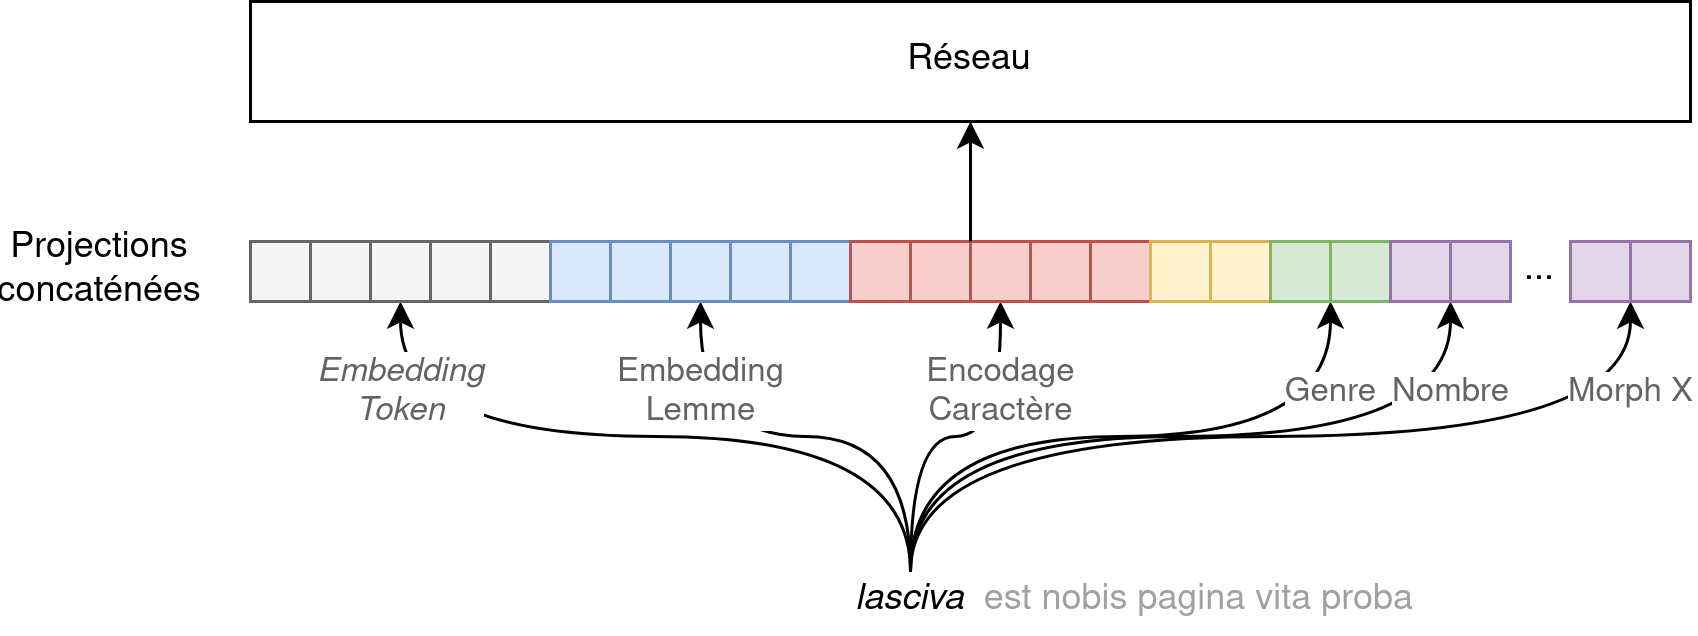
\includegraphics[width=\linewidth]{figures/chap4/Projection.drawio.png}
    \caption{Projection maximaliste réutilisant l'ensemble des informations à disposition du modèle (forme, lemme, caractère, traits morphologiques, POS): chaque information est toujours insérée dans le même ordre.}
    \label{fig:chap4:projection:morphosyntax}
\end{figure}
% ~  < 1 page ? (un gros paragraphe)

% POS et héritage des différentes problèmes cités plus hauts sur lemme / forme et perte d'information
% Problème des embeddings avec le mot

\subsubsection{Intégration des métadonnées}
\label{chap4:encodage:metadonnees}

\enquote{[Quand] la métaphore [est] \textit{in absentia}, elle instaure une connexion symbolique qui doit être identifiée par des conjectures concordantes sur le discours, le type de l'œuvre, le genre du texte, la hiérarchisation idiolectale des isotopies.\footcite[p. 98]{rastier_tropes_1994}}. Ces seuls mots de F.~Rastier indiquent ô combien la question du contexte est importante dans notre cas. Non content d'avoir dans nos textes de très nombreux passages du lexique de la sexualité, sur lesquels la machine ne devrait pas buter, la question de la métaphore et en général des tropes risque de se heurter à un mur: la machine ne connait pas ce que Martial est à la littérature latine, mais ne sait pas non plus, si on ne l'informe pas, que \enquote{\textit{Lasciva est nobis pagina}} est de Martial. La formalisation de ce contexte, de ces métadonnées, est alors répartie sur deux niveaux: un premier niveau qui concerne le document, l'œuvre (auteur, siècle, etc.) mais nous proposons de distinguer un second niveau, celui des \enquote{métadonnées de mots} (propriétés extra-linguistiques entre autres).

La problématique du contexte et de sa formalisation est encore assez récente dans les travaux de classification et de traitement séquentiel du langage en général. Parmi les rares publications existantes sur le sujet, on note celle de J. Kim et al.\footcite{kim_categorical_2019}. Les auteurs de cet article ajoutent l'information en parallèle au texte, en testant plusieurs moments d'insertion: les métadonnées sont d'abord projetées puis intégrées via des modifications de réseaux ou des concaténations. Le principe qui sous-tend cette insertion de la métadonnée par J. Kim est celui des goûts propres à un locuteur: cherchant à évaluer des critiques (culinaires en autres), les particularités de chaque locuteur peuvent s'exprimer à travers une relation lexique-évaluation notée. Ainsi, si une personne donne des critiques négatives en utilisant le terme \textit{épicé}, il est possible que ce terme ne relève pas des informations positives et aide à classer de futures des remarques. En ajoutant l'information liée à l'identité du locuteur, les auteurs montrent une augmentation du score atteignant jusqu'à +4.45 points de pourcent de la classification: la machine se met à prendre en compte l'idiolecte dans sa classification\footnote{L'exemple donné relève principalement de la partie lexicale d'un idiolecte, mais il est possible aussi que des faits de syntaxes puissent trahir les particularités propres de chaque critique.}.

% HERE 
Au-delà de l'intégration de l'idiolecte, la question du sociolecte peut-être tout aussi importante: \textit{virgo} n'a pas la même valeur pour un Romain chrétien et un romain païen, pour un romain du IVe siècle et du IIe d'avant notre ère. On retrouve d'ailleurs un usage des particularités d'un sociolecte dans l'une des études précédemment citées, celle de \textit{bot.zen}, où les chercheurs ont utilisé des plongements de mots dérivés de textes écrits par des apprenants de la langue anglaise\footcite{stemle_using_2018}. L'usage pour les plongements de mots d'une contextualisation temporelle\footcite{carlo_training_2019} ou géographique liées au contexte\footcite{gong_enriching_2020} n'est pas rare, contrairement à son utilisation dans des tâches de classification. Parmi les études sur l'usage de ces données, celle de Huang et Paul\footcite{huang_neural_2019} a la particularité de mettre au banc d'essais l'influence de l'injection de métadonnées temporelles dans les données pour des tâches de classification sur les sets habituels d'Amazon, Yelp, etc. Sur l'espace de trois à plus de dix ans, ils montrent et quantifient l'existence de changements de contexte et de déplacements sémantiques dans les datasets. L'usage d'informations temporelles montre une amélioration dans tous les cas, avec des augmentation de l'\textit{accuracy} allant d'un négligeable +0.4 à un impressionnant +3.8 points.

Enfin, il existe un dernier type d'information, en partie sociolectale, qui ne semble pas avoir intéressé outre mesure: celui de la prise en compte des \textit{sèmes} liés aux entités nommées, à savoir les lieux, les personnes, les divinités, les organisations, etc. Quand un romain parle d'Athènes, ou de Troie, un ensemble de sèmes peuvent apparaître: /Grèce/, /Épopée/, /Philosophie/, etc. Ces informations ne sont pas toujours déductibles des co-occurrences - tous les locuteurs ne font pas comme les Américains en indiquant l'état dans lequel une ville se trouve (\enquote{Austin, Texas}), et encore, ce phénomène est réservé aux villes nord-américaines - et peuvent relever d'une projection géographique, historique, littéraire - les prostituées ont des noms grecs à Rome: qu'est-ce qu'un nom grec pour la machine ? Cette connaissance des propriétés des personnes (Martial et Sénèque viennent des régions espagnoles, Sénèque est un \enquote{conseiller politique} via sa position auprès de Néron), des lieux (localisation géopolitique) et des auteurs (Martial et Sénèque sont des auteurs dans des genres différents) ne peut transpirer entièrement et assez régulièrement pour que ces sèmes soient présents associé à leur nom. Les \textit{embeddings} étant une représentation de l'espace sémantique, des études pour fusionner des graphes de connaissances \enquote{encyclopédiques} avec ces derniers existent, qu'il s'agisse d'\textit{embeddings} classiques\footcite{wang_knowledge_2014} ou contextuels\footcite{zhang_ernie_2019}, mais leur application au latin semble encore assez lointaine. Dans \enquote{\textit{Semantic structure-based word embedding by incorporating concept convergence and word divergence}}\footcite{liu_semantic_2018}, Liu et ses collègues utilisent dans leur entraînement d'\textit{embeddings} un second objectif, celui de réduire la distance entre synonymes, hyponymes et hyperonymes issus d'un \textit{WordNet}: les gains en classification sur un corpus de presse dépassent leur meilleure \textit{baseline} de +0.4\% de score F1. Si un tel gain peut paraître minime, la limitation à un graphe sémantique tel que WordNet nous paraît dommage, surtout dans le cadre d'une classification d'articles de journaux, leur terrain d'expérimentation, où la relation entre entités nommées et leur classification ne peuvent être extraites du dictionnaire.


\subsection{Modèles et variations de modèles}

La construction du modèle pour cette recherche repose sur une architecture modulaire, permettant de tester de nombreuses hypothèses, tant du point de vue des modules d'encodage que des informations conservées. Du point de vue technique, l'ensemble de ces modèles sont construits sur la même architecture, avec des variations afin d'évaluer les apports des différentes informations et divers réseaux. Le plan du modèle est découpé en trois blocs principaux: 
\begin{itemize}
    \item un bloc de projection, qui vise à représenter chacune des unités d'information (mot, information morphologique, POS, métadonnée, etc.) dans l'espace;
    \item un bloc d'encodage, qui cherche à représenter le texte;
    \item une couche décisionnelle, qui produit la classification.
\end{itemize}
En fin de modèle, suivant qu'il s'agisse d'un entraînement ou d'un moment de prédiction, on trouvera une transformation de la décision en perte (\textit{loss}) ou en classification. Cette architecture est commune à l'ensemble des différents modèles étudiés jusqu'ici et nous permet d'y étudier des variations (\textit{cf.} Figure \ref{fig:chap4:Architecture}).

\begin{figure}
    \centering
    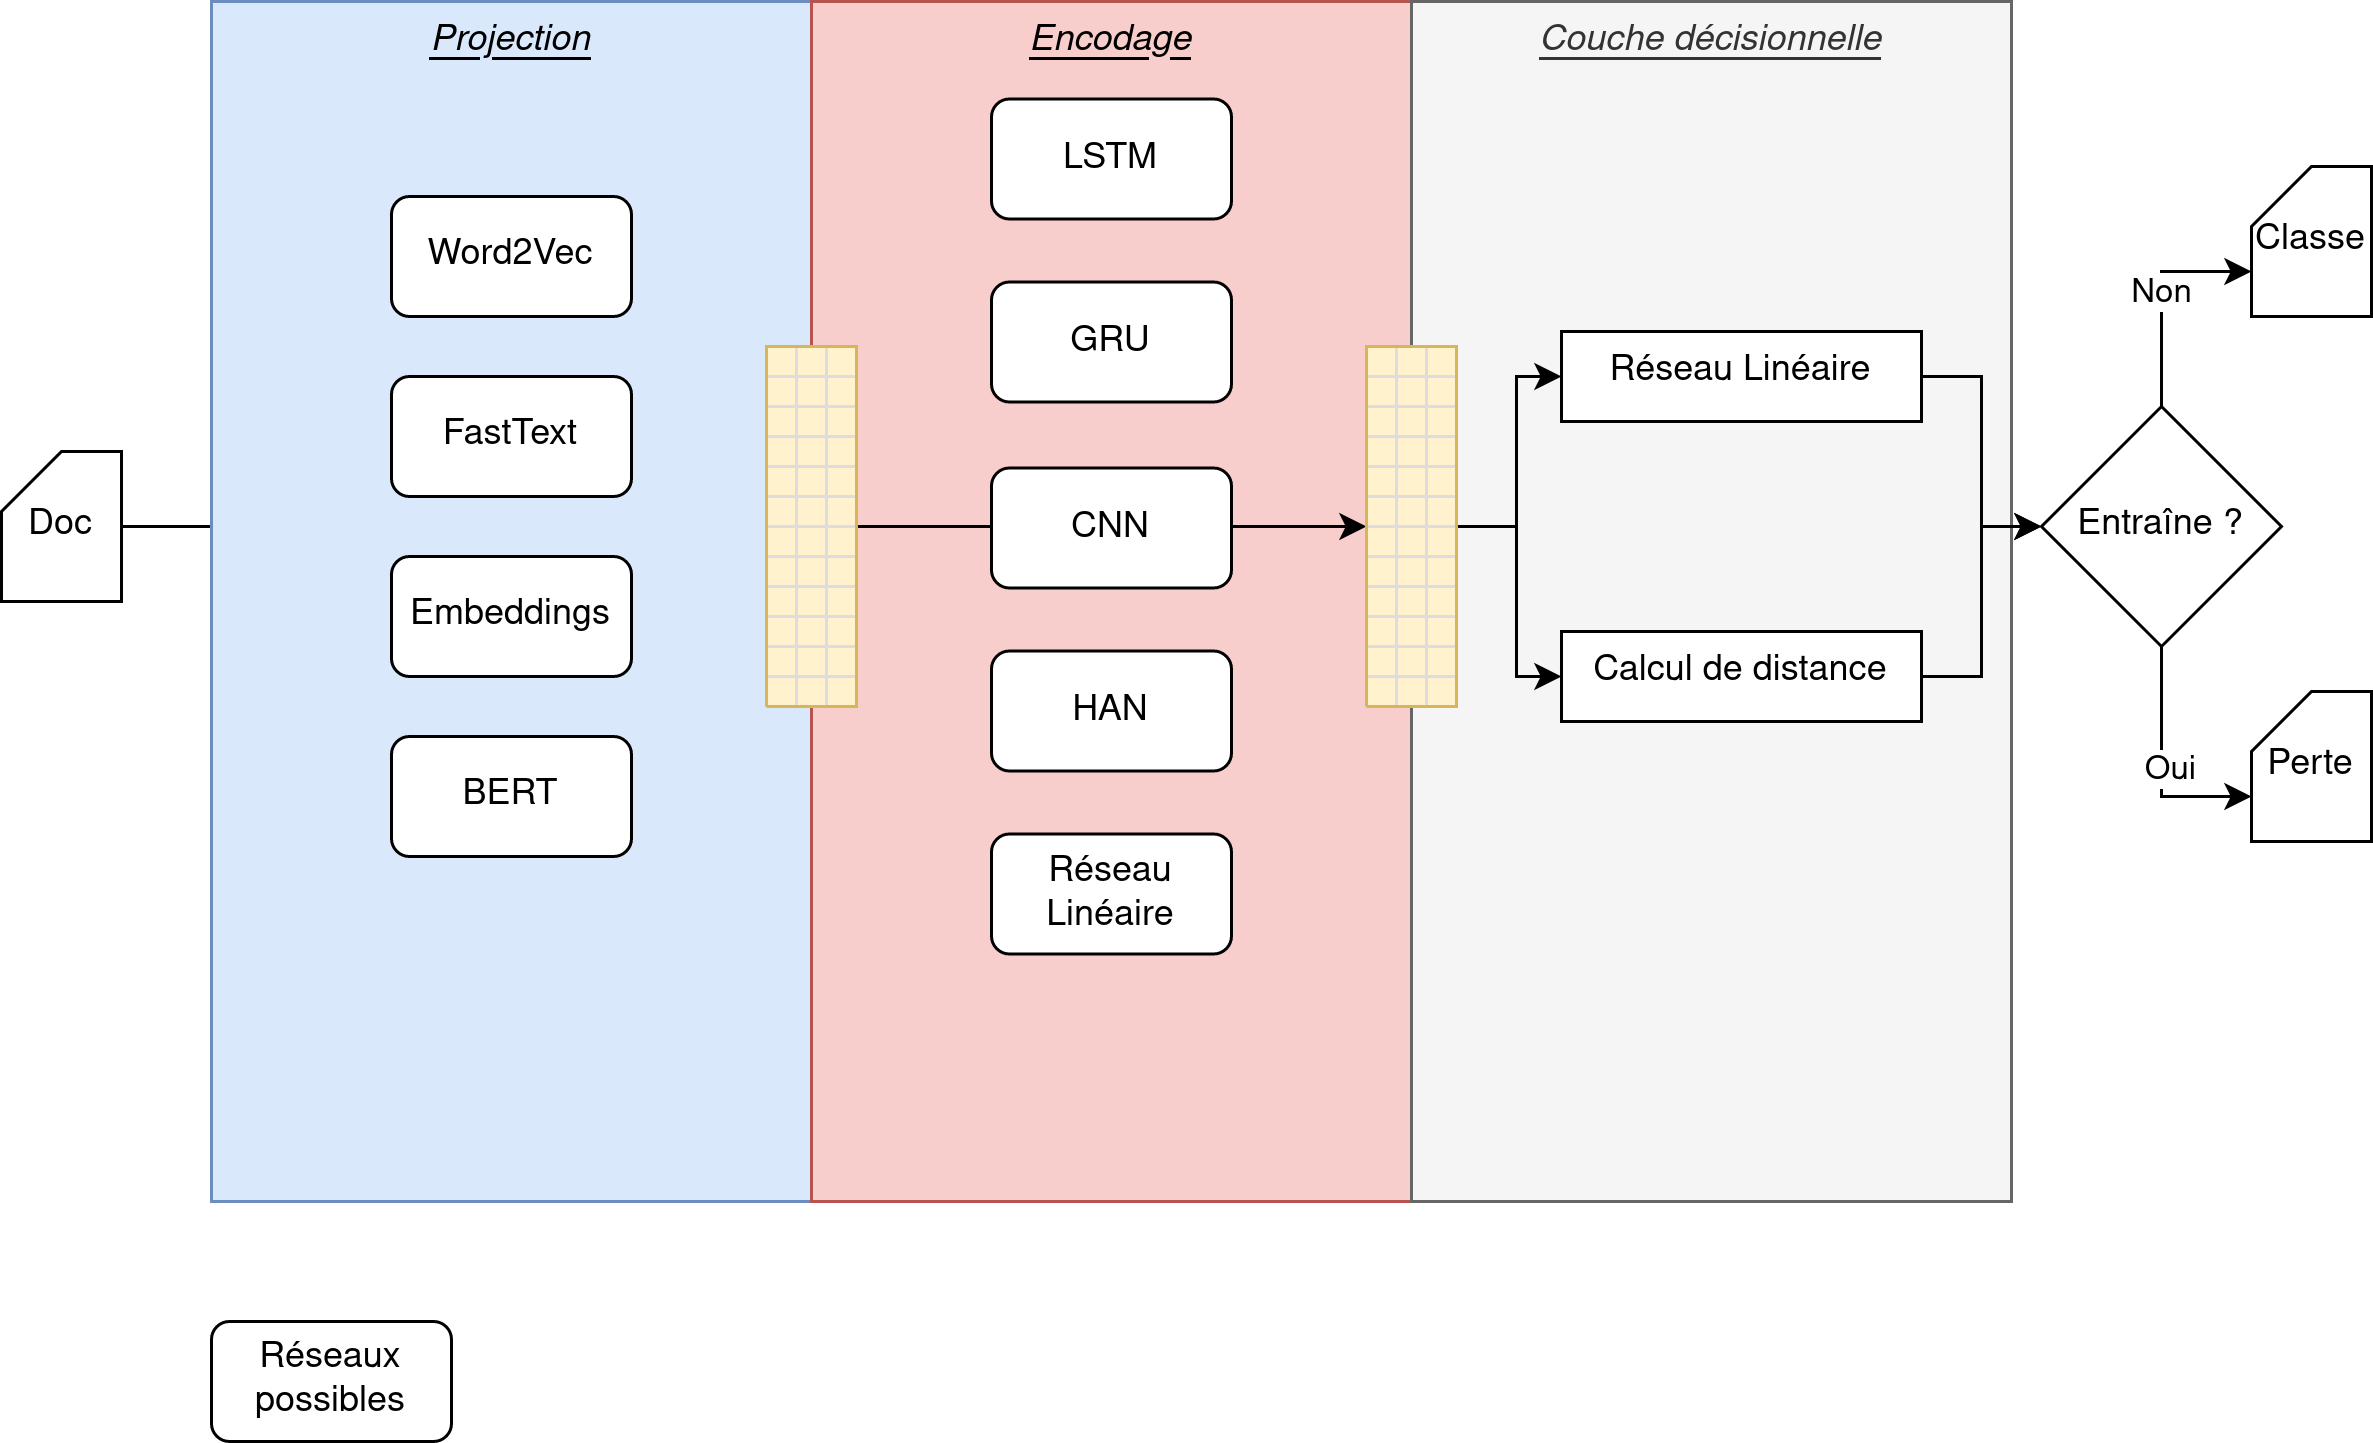
\includegraphics[width=\linewidth]{figures/chap4/architecture.png}
    \caption{Découpage de l'architecture générale. On distingue trois étapes: le passage des mots à des projections au niveau token, leur encodage au niveau phrase puis la partie de prise de décision. Selon que l'on entraîne ou que l'on utilise l'outil pour des prédictions, on obtient un score de perte ou de classification. Plusieurs modèles sont utilisables pour les deux premières couches de l'architecture.}
    \label{fig:chap4:Architecture}
\end{figure}

\subsubsection{Le bloc de projection}

La première forme de transformation s'effectue au niveau des tokens produits par \textit{Pie-Extended}: la séquence de tokens est fournie au modèle, qui utilise ou non l'ensemble des informations disponibles, à savoir les informations morphosyntaxiques, de formes ou de lemmes. Les formes et lemmes sont projetés par des embeddings pré-entraînés via Gensim\footcite{gensim} et non-entraînables basés sur \textit{FastText} ou \textit{Word2Vec} et de taille 200. Les catégories individuelles de morphosyntaxe (\texttt{Cas=X}, \texttt{Genre=X}, etc.) sont projetées sur une dimension assez faible de 3, tandis que la concaténation de ces tags (\texttt{Cas=X|Genre=Y}) est projetée sur une dimension de 20. En cas de projection au niveau caractère, disponible pour les lemmes et les formes, afin de prendre en compte la morphologie flexionnelle pour les caractères et les morphèmes non-flexionnels pour les deux, on utilise un encodage au niveau caractère utilisant un réseau LSTM avec une \textit{hidden size} de 150, deux couches et un \textit{dropout} de 30\%. L'ensemble des projections est concaténée en un seul vecteur pour chaque token (\textit{cf.} figure \ref{fig:chap4:projection:morphosyntax}).

On peut ajouter à cette transformation des formes, lemmes et informations morphosyntaxique un encodage via le module Bert latin, développé par D. Bamman et P. J. Burns. Deux problèmes se sont posés avec cette utilisation, dont un n'a pu être résolu. D'une part, le module pose un problème d'ingénierie: l'outillage entourant le modèle Bert est peu documenté, lent et repose sur des versions plutôt anciennes de certains outils qui ont parfois été un véritable puzzle de dépendances\footnote{CLTK posant notamment de gros problèmes sur ce point.}. Ensuite, il y a un véritable problème dans le pré-traitement de l'information: les deux auteurs du projet ont utilisé la tokenisation de CLTK en pré-traitement, que nous avons voulu à tout prix éviter, car, basée sur des règles, elle a une forte propension à interpréter chaque morphème final \textit{-ne} comme un clitique, de même que les \textit{-ve} ou les \textit{-que} (par exemple, \textit{observatio-ne} et \textit{observatio-ve} sont systèmatiquement tokenizés en deux morceaux, bien que le premier est souvent un simple ablatif). L'usage de ce \textit{pre-tokenizer} est par ailleurs une bizarrerie algorithmique du point de vue de Bert: l'objectif même de ce dernier, avec ses systèmes de tokenization reposant sur des \textit{sous-tokens}, est de pouvoir gérer ce type de phénomènes. Par exemple, dans le cadre du modèle Bert allemand de Chan et al.\footcite{chan_german_2019}, on retrouve ainsi logiquement traités par le \textit{tokenizer} les sous-tokens grammaticaux \texttt{\#\#ge}, les préfixes \texttt{\#\#be} et \texttt{\#\#ver}, sans pré-traitement manuel par les chercheurs: \textit{vergenommen} est ainsi transcrit en \texttt{\#\#ver + \#\#genommen}\footnote{\textit{nehmen} ayant de nombreux dérivés et étant relativement fréquent dans la langue allemande, il n'est pas étonnant que le composant \texttt{\#\#genommen} existe permettant ainsi une construction économique en bi-gram pour \textit{abnehmen, vernehmen, etc.}}. Nous nous sommes ainsi refusé à utiliser la prétokenization faussée de CLTK, espérant que le composant de tokenization de Bert soit suffisant pour pallier à cette situation\footnote{Mais la différence de tokenization pousse tout de même au final à l'incapacité d'aligner - simplement - les tokens.}. Enfin, en cas d'usage de projections via Bert et de projection classiques par \textit{embeddings} non contextuels, on utilise soit une concaténation des vecteurs Bert avec les vecteurs issus des plongements non contextuels, soit une réduction via une réduction en réseau linéaire.

\subsubsection{Le bloc d'encodage}

Le bloc d'encodage est probablement le plus simple des trois blocs. Il prend comme entrée les projections unitaires précédentes - au niveau token - pour produire une projection séquentielle - au niveau texte. On utilise majoritairement dans ce contexte des réseaux récurrents, LSTM et GRU, en mode bi-directionnel, avec un \textit{dropout} de 30\% et et une taille de 50 par direction. Alternativement aux réseaux récurrents, on retrouve aussi une option pour un réseau convolutionnel, avec des tailles de filtres de 2 à 5 (n-grams) et 5 filtres, un filtrage par MaxPool et une activation par ReLU.

Si ces réseaux sont communs, la recherche en classification a fait émerger d'autres moyens d'obtenir une représentation en augmentant ces modules. Le plus important de ceux-ci est sans aucun doute celui décrit dans \textit{Hierarchical Attention Networks for Document Classification}(\textit{HAN})\footcite{yang_hierarchical_2016}, présenté en 2016, basé sur des réseaux récurrents et qui sera décliné avec un modèle convoluttionnel (CHAN) en 2019\footcite{gao_hierarchical_2018}. Le principe d'\textit{attention} qu'il intègre et qui essaye de tirer d'une séquence les unités les plus importantes dans le cadre d'une classification, permet de pondérer ces unités dans le cadre de l'encodage de cette séquence. Par exemple, dans \textit{Lasciva est nobis pagina, vita proba}, dans le cadre de notre recherche, les mots présentant l'isotopie de la sexualité pourraient être en premier lieu \textit{lasciva} puis, peut-être, \textit{proba}, dans son jeu d'opposition /lascif/ contre Non(/lascif/). Les termes \textit{vita} et \textit{pagina} n'ont pas ou peu d'importance directe pour notre sujet, tandis que \textit{est}, \textit{nobis} et les signes de ponctuation n'en ont absolument aucune à priori. Cette importance des termes se traduit par une attention forte, tandis que le caractère négligeable des autres unités se traduit par une attention quasi-nulle.

Ce complément pour l'encodage séquentiel a aussi l'avantage de fournir au lecteur un outil d'analyse de ce qu'apprend le modèle. En ajoutant aux informations classiquement produites par le modèle, telles la classification les pondérations de l'attention, il met en exergue les traits saillants détectés. Cet outil a deux intérêts majeurs. D'une part, à travers les jeux de répétition qui auraient échappé à l'œil humain, il peut permettre de questionner une analyse plus manuelle des sèmes actualisés par une isotopie: les mots portants ces sèmes sont identifiés par le phénomène d'attention et amènent à interroger leur rôle. D'autre part, il peut permettre de détecter des phénomènes que nous qualifierions de \enquote{triche} mais qui relève bien du sur-apprentissage: dans notre cas, il nous est arrivé de trouver que pour les textes d'une édition en particulier, l'obèle de l'édition était un token spécifique au corpus positif, que le modèle a ainsi interprété comme trait saillant. Ce phénomène peut se retrouver avec d'autres mots, dont les actualisations /sexuel/ ne sont pas les plus courantes: c'est à cet endroit que l'équilibrage du corpus est important.

Dans le cadre de notre usage de Bert, il existe deux situations: une première où Bert est la seule projection utilisée, une second où Bert est employé avec d'autres projections.

Pour la première des deux, il existe plusieurs stratégies, dont la plus commune consiste à exploiter les tokens de délimitation des phrases \texttt{[CLS]} et \texttt{[SEP]} qui représentent respectivement le début de la séquence et la fin de la séquence. Bert proposant des plongements de token contextualisés, ces deux éléments ont la particularité de contenir une information contextualisée sur la phrase sans porter eux-mêmes de signification propre. Parmi les autres stratégies, on distingue les fonctions de réduction par moyenne (\textit{Reduce Mean}) et par valeur maximum (\textit{Reduce Max}), ainsi qu'une combinaison des deux via concaténation. Bert étant son propre réseau neuronal avec plusieurs couches, certains chercheurs et services recommandent d'éviter d'utiliser la dernière couche si il n'y a pas de ré-entraînement\footnote{\textit{Cf.} \url{https://github.com/hanxiao/bert-as-service/blob/master/docs/section/faq.rst\#bert-has-12-24-layers-so-which-layer-are-you-talking-about}}: elle serait ainsi trop liée à l'objectif initial de Bert (prédiction de mot ou de phrase suivante) et servirait donc de mauvaise ressource pour des tâches différentes. Afin d'ajouter une couche d'entraînement supplémentaire, on peut passer cette représentation via Bert dans un réseau ayant pour objectif de réduire l'information (couche linéaire): ainsi, d'un vecteur de 768 ou 1536 (\textit{MeanMax}) on passe alors à 256 avant d'entrer dans le bloc décisionnel. Il est aussi possible d'utiliser la projection contextualisée dans des réseaux plus traditionnels, tels que GRU, HAN ou LSTM.

\begin{figure}[ht]
    \centering
    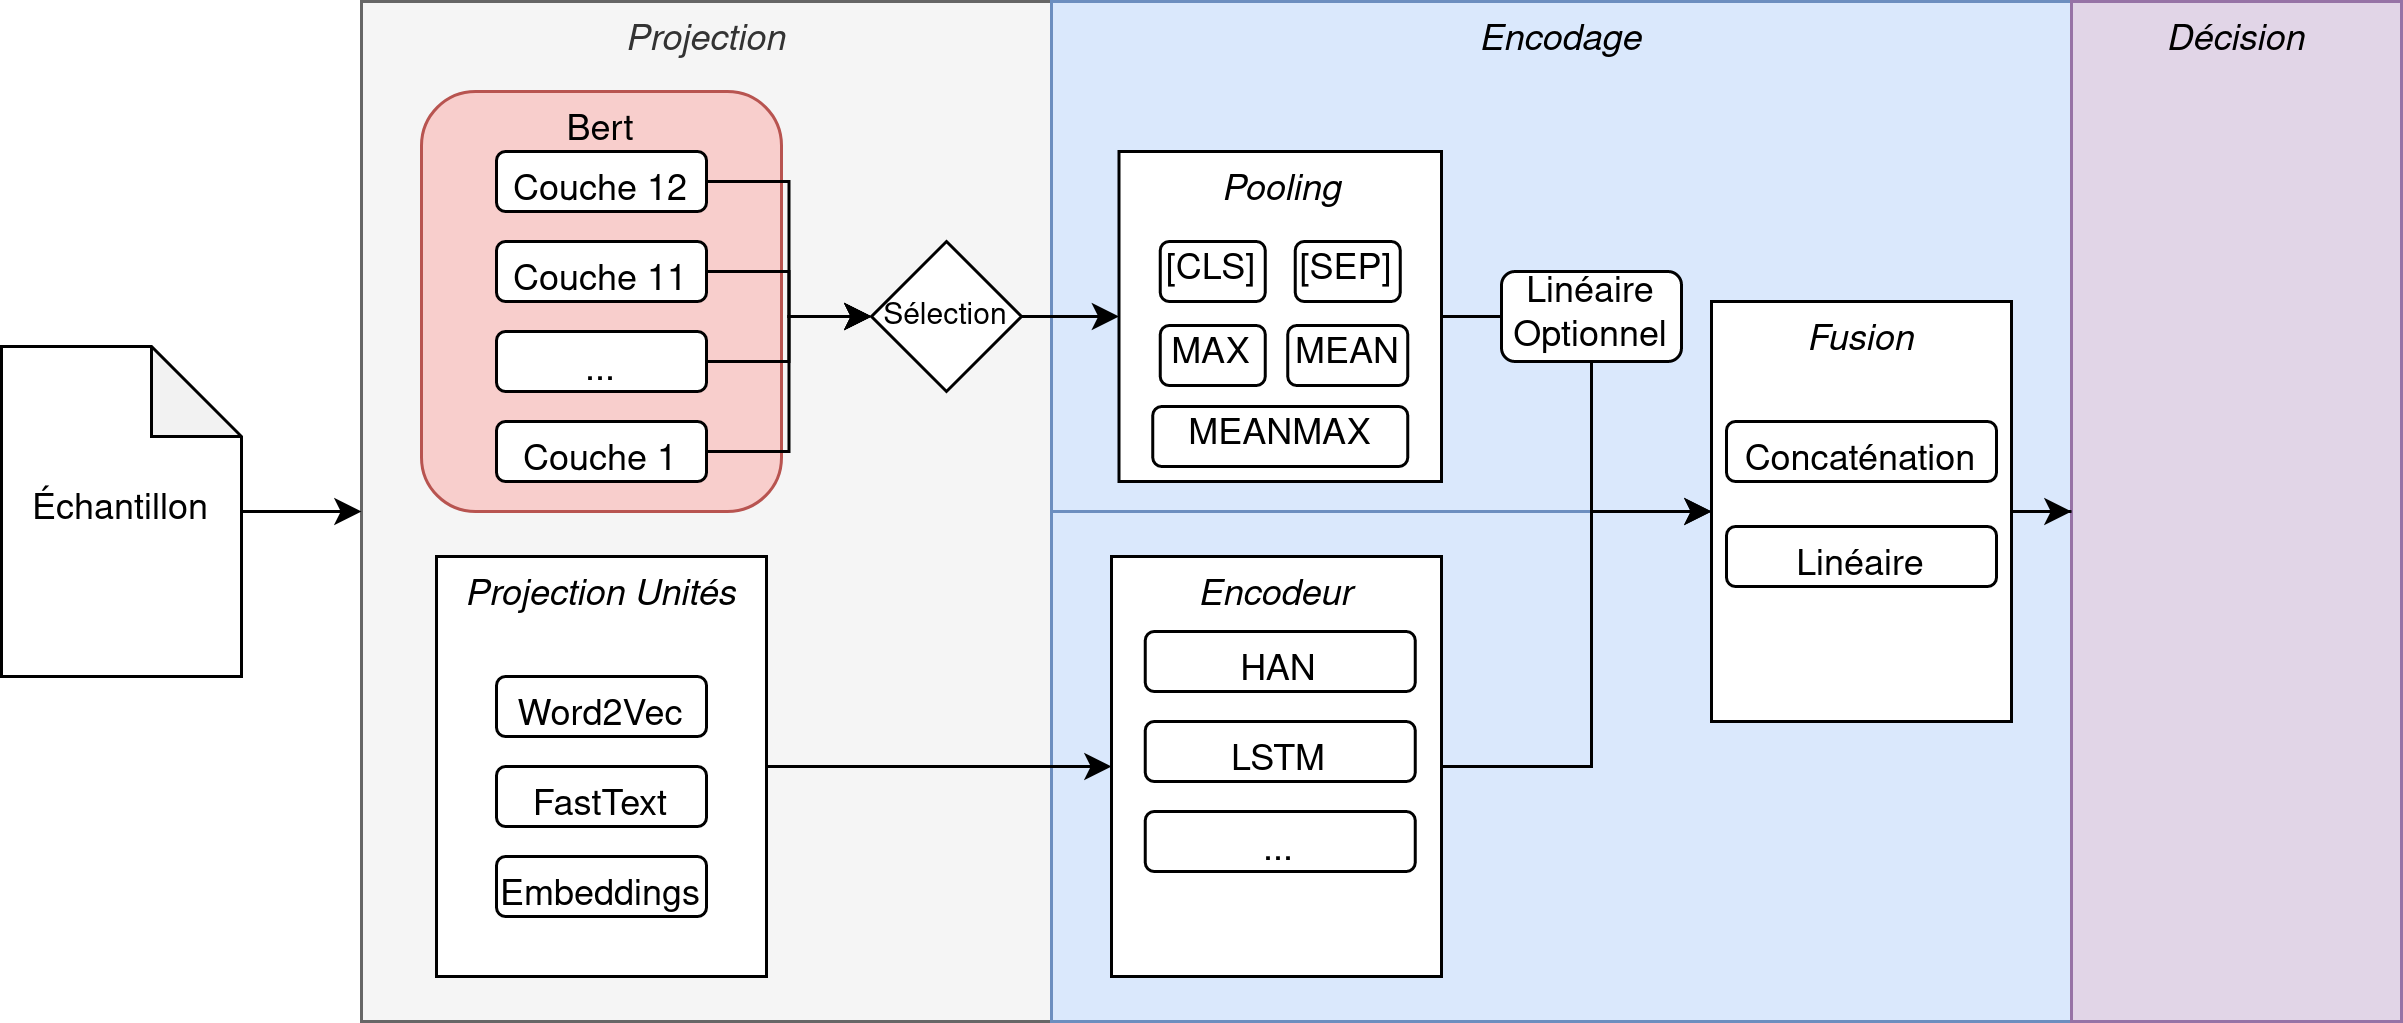
\includegraphics[width=\linewidth]{figures/chap4/BertZoom.png}
    \caption{Zoom sur les possibilités et relations entre projection et encodage.}
    \label{fig:chap4:zoom-projection}
\end{figure}

Pour le second cas, où projections par Bert et projections par embeddings non-contextualisés se complètent, on procède ainsi: la projection de Bert est effectuée comme dans le cas précédent via une méthode de \textit{pooling} et une optionnelle réduction linéaire, tandis que la projection traditionnelle est encodée via l'un des réseaux décrits plus hauts, récurrent ou convolutionnel. Les deux entrées sont ensuite ou concaténées, ou réduite via une couche linéaire, afin de fournir les deux informations (\textit{cf.} figure \ref{fig:chap4:zoom-projection}).

\subsubsection{Classification, similarité: la couche décisionnelle et les méthodes d'entraînement}

Après avoir projeté les unités et encodé la séquence, le modèle passe à la dernière phase de la classification, celle de la couche décisionnelle. Cette couche décisionnelle se décline en deux architectures principales: l'une, classique, orientée classification via une projection linéaire; l'autre, plus particulière, orientée comparaison.

La première architecture est assez simple: elle prend en entrée l'information encodée par le bloc précédent et, via une couche linéaire, réduit celle-ci en un vecteur de taille 2, où chacune des cordonnées du vecteur représente une classe, ici \texttt{isotopie sexuelle} ou \texttt{absence de cette isotopie}. Pour produire la classification, on applique au vecteur une fonction \textit{softmax}, qui a la particularité d'équilibrer les valeurs telles que la somme des valeurs du vecteur soit égale à 1 en conservant la hiérarchisation des valeurs (le score le plus haut reste le plus haut). Pour la perte, on applique une traditionnelle \textit{Cross Entropy Loss}.

La seconde architecture est plus complexe, car elle recoupe plusieurs variations. Son principe fondamental est de comparer la sortie du bloc d'encodage - donc l'échantillon encodé - avec un ou plusieurs échantillons encodés dont la classe est connue. Cette méthode, dite de réseau siamois, consiste donc à faire passer dans le même réseau les données et d'inférer une classe en fonction de la proximité d'un texte avec un ou plusieurs autres textes. 


\begin{figure}[ht]
    \centering
    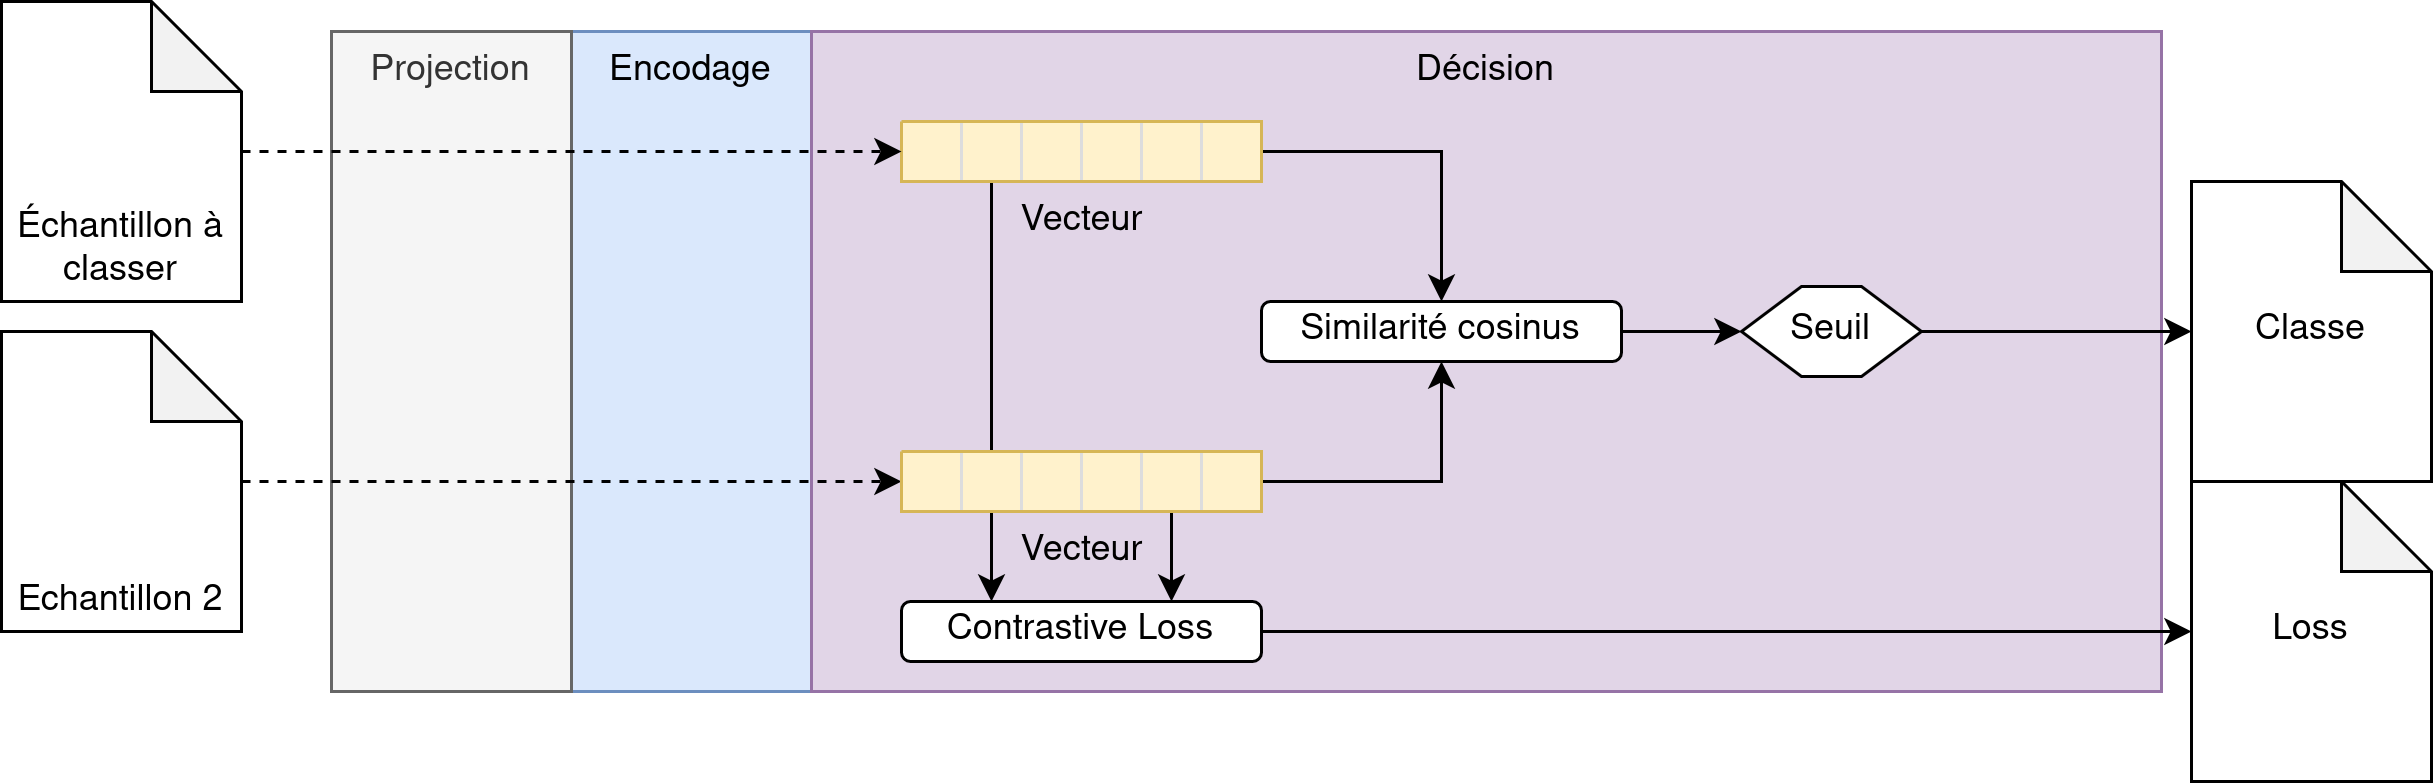
\includegraphics[width=\linewidth]{figures/chap4/contrastive.png}
    \caption{Schéma de fonctionnement d'un réseau siamois à double échantillons.}
    \label{fig:chap4:reseau:ContrastiveLoss}
\end{figure}

La première variation des réseaux siamois utilise deux échantillons, un que l'on souhaite classer, et un dont on connait la classe, ci-après le comparant. Une fois encodés, on les compare à l'aide d'une fonction de similarité cosinus: si la similarité entre les deux dépasse un seuil, fixé arbitrairement pour nous à 0.6, l'échantillon est considéré comme appartenant à la classe du comparant. Au contraire, si le seuil n'est pas atteint, cette appartenance est rejetée. Pour la perte (\textit{loss}), qui permet de diriger l'entraînement, on utilise une \textit{contrastive loss}\footcite[Entre autres, ]{khosla_supervised_2021} qui prend directement comme paramètres les encodages d'échantillons pour calculer un écart entre les deux (\textit{cf.} image \ref{fig:chap4:reseau:ContrastiveLoss}). La seconde variation des réseaus siamois utilise trois échantillons, dont deux comparants. Ces deux échantillons de comparaison ne doivent pas représenter la même classe, et l'un d'eux doit, au possible, avoir la même classe que celui avec lequel on entraîne le modèle. On calcule la distance entre les comparants encodés et l'échantillon via une distance euclidienne, et l'on attribue la classe du comparant le plus proche à l'échantillon évalué. Pour la perte, on utilise une perte appelée \textit{Triplet Margin Loss}\footcite{hermans_defense_2017} qui est alors calculée directement à partir des données issus de la phase d'encodage.

\begin{figure}[ht]
    \centering
    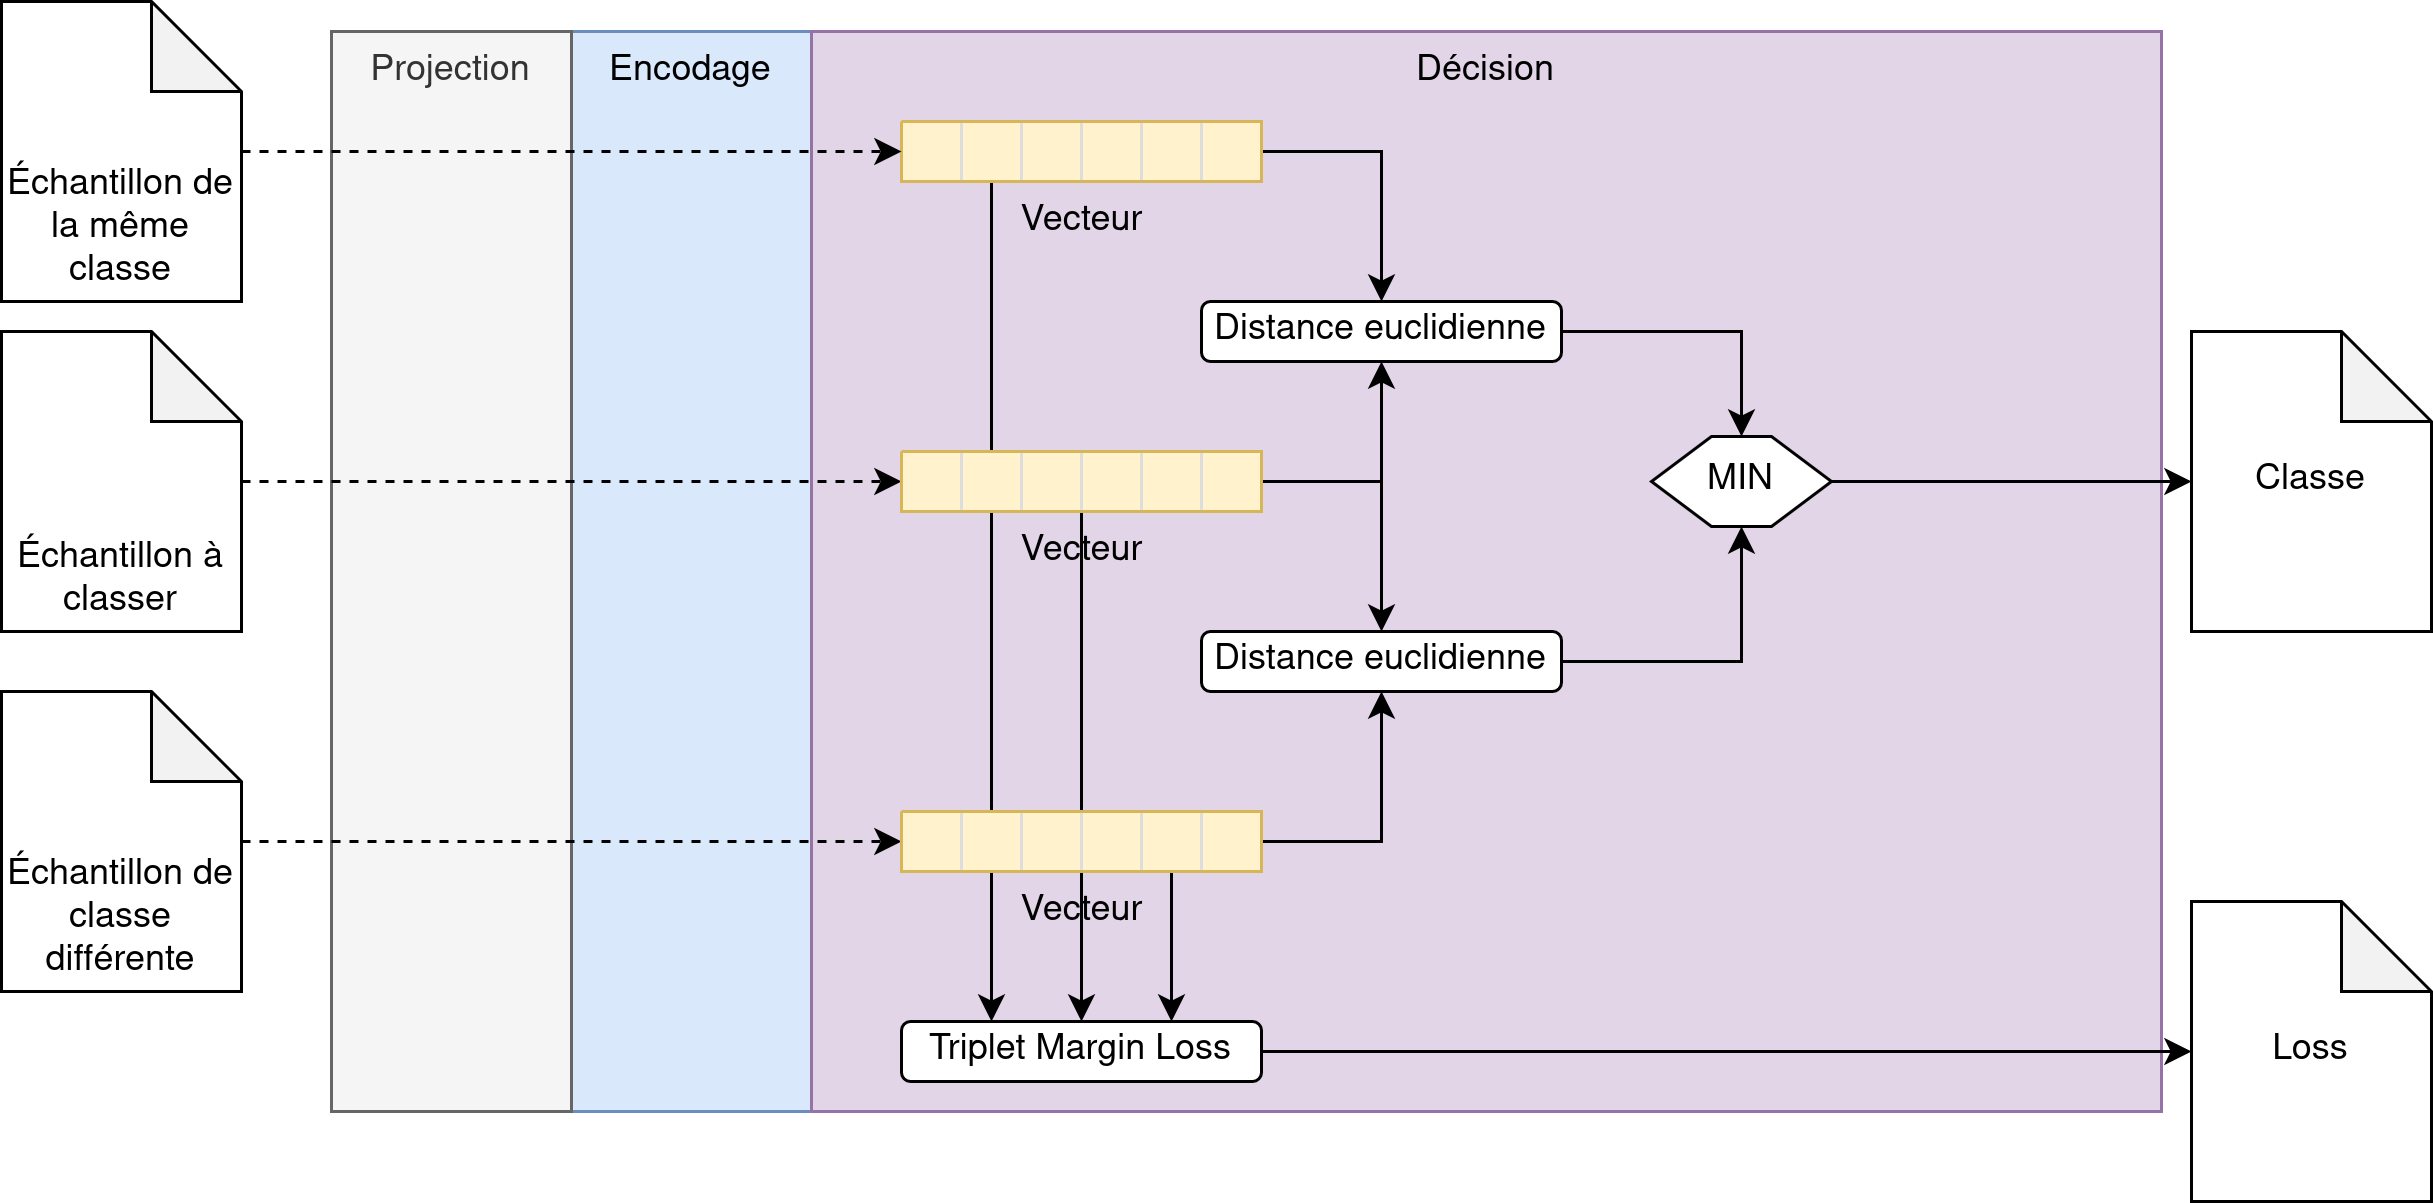
\includegraphics[width=\linewidth]{figures/chap4/triplet.png}
    \caption{Schéma de fonctionnement d'un réseau siamois à triple échantillons.}
    \label{fig:chap4:reseau:Triplet}
\end{figure}

Pour ces deux variations, les stratégies d'entraînement ou de prédiction peuvent varier. La méthode la plus simple, à la fois algorithmiquement et méthodologiquement, est la sélection manuelle d'un ou plusieurs représentant(s) par classes: à chaque fois que le modèle entraîne un échantillon, il tire au hasard un représentant positif ou négatif avec lequel les distances seront calculées. Ces représentants sont ensuite sauvegardés avec le modèle afin de pouvoir continuer à effectuer des prédictions. Une autre méthode d'échantillonnage consiste à prendre tous les binômes ou triplets possibles d'un même ensemble d'échantillons et de les utiliser comme données à évaluer. Il existe cependant des méthodes d'échantillonages qui cherchent à mathématiquement maximiser les erreurs afin de rendre l'apprentissage le plus difficile possible, nous en testons deux: le \textit{BatchEasyHard} de Xuan et al.\footcite{xuan_improved_2020}, qui cherche à trouver des triplets dont le comparant positif est simple mais le comparant négatif est complexe, et le \textit{BatchHard} de Hermans et al.\footcite{hermans_defense_2017} qui cherche par défaut les triplets les plus complexes à classer pour chaque échantillon\footnote{Nous utilisons les implémentations de ces échantillonneurs issu es de la librairie \texttt{pytorch-metric-learning}, \cite{musgrave2020pytorch}}. 
\subsubsection{Le cas particulier de l'inclusion des métadonnées}

Nous parlions en \ref{chap4:encodage:metadonnees} de la possibilité et de la potentielle importance d'incorporer les métadonnées en tant qu'elles apportent des identificateurs extra-linguistiques pour les idiolectes et sociolectes. Nous approchons le problème de deux manières différentes: d'une part, à travers l'intégration de tokens de métadonnées dans la séquence, d'autre part via l'utilisation de modules modifiés en suivant les travaux de \footcite{kim_categorical_2019}. Quatre domaines de métadonnées peuvent être injectés, à savoir: la période d'écriture (le siècle), l'auteur, la structure logique de citation (par exemple: chapitre,section) et la forme d'écriture (prose ou vers).

Dans le cas de token de métadonnées, les vecteurs de mots sont nécessairement entraînables et non figés par le pré-entraînement, et on ajoute au vocabulaire des ces différents modèles de de nouveaux éléments suivants une syntaxe spécifique, telle \texttt{$[$Date:1$]$}. Ces tokens sont traités sans POS et sans morphologie, leur lemme étant identique à leur forme. Ils sont ensuite traités comme le reste des tokens par les réseaux d'encodage.

Dans le second cas, les métadonnées sont projetées dans des espaces propres de taille 64 comme des embeddings. Ces données sont ensuite injectées dans des modules modifiés: nous proposons ainsi, grâce aux travail de Kim et al. des modifications des réseaux LSTM, HAN basé sur LSTM et de la couche linéaire pour la partie décisionnelle. De même que dans l'article original, cette information ne peut être injectée qu'une seule fois dans le réseau par échantillon.

\section{Les modèles obtenus}

L'entraînement de modèles et la construction d'architectures est un processus itératif: il s'agit de tester des hypothèses de modèles, des hypothèses de paramétrages de modèles, puis d'aller dans l'une ou l'autre direction qui semble apporter les meilleurs réponses. Rendre compte de ce processus, et de ses résultats, n'est pas une mince affaire: la chronologie a un rôle dominant dans la sélection de modèles qui iront jusqu'au bout.

\subsection{Résultats principaux}

% Commencer par les métadonnées en fait
% Ensuite, séparer Bert et Non Bert

% Expliquer itération: un run par archi. d'abord, pour évacuer les mauvaises archis.

\subsubsection{Le problème des métadonnées \textit{auteur} et \textit{structure éditoriale}}

% Dans une première salve d'entraînement, ceux-ci performent le mieux. Quelques scores

% MAIS c'est du sur-apprentissage: si on applique le modèle en mode prédiction, on se rend compte que TOUT Martial est tagué en positif, mais quand il dit bonjour.

\subsubsection{Bert: formes d'usage}

% Ré-entraînement = 0
% Ok, les méthodes Bert sous performent malgré ce que promet la littérature vue plus haut.
% Mais quid d'autres méthodes de Pooling ?

\subsubsection{Les modèles linéaires}

% Ouai mais ça c'est top

% Test des différentes méthodes de Pooling, confirme les avis de plus haut

% Test des méthodes RNN: beaucoup plus intéressant

% Paragraphe sur incapacité de compléter l'alignement tok+subword


Une méthode peut apporter de premiers très bons scores puis, sur le terrain, montrer de très grosses faiblesse, via un problème de surapprentissage. Au

\subsubsection{L’échec des modèles de similarité}

% Pourquoi le mining n’apporte rien ?

\subsection{Extensibilité des modèles}

\subsubsection{Impact de la taille du dataset: random petit}

\subsubsection{Entraîner à partir de termes explicites uniquement}

%mentula, cunnus, pedico, futuo, culus ?

\subsubsection{Entraîner à partir de métaphores uniquement}

\subsection{Ce qu’apprend le modèle?}

\subsubsection{Comparer “l’attention” en fonction des modèles}

%Note pour moi-même: Max(attention) similaire par modèle est-elle toujours la même ?

\subsubsection{Analyse des erreurs des X meilleurs modèles}

%Erreurs les plus fréquentes: Quels tags ? Quels mots ?

%Classification des types d’erreurs

%	Sur-apprentissage (Martial == Sexe)

%	Sous-apprentissage (Termes de la guerre =? Sexe)

